% Options for packages loaded elsewhere
\PassOptionsToPackage{unicode}{hyperref}
\PassOptionsToPackage{hyphens}{url}
%
\documentclass[
]{article}
\usepackage{amsmath,amssymb}
\usepackage{lmodern}
\usepackage{iftex}
\ifPDFTeX
  \usepackage[T1]{fontenc}
  \usepackage[utf8]{inputenc}
  \usepackage{textcomp} % provide euro and other symbols
\else % if luatex or xetex
  \usepackage{unicode-math}
  \defaultfontfeatures{Scale=MatchLowercase}
  \defaultfontfeatures[\rmfamily]{Ligatures=TeX,Scale=1}
\fi
% Use upquote if available, for straight quotes in verbatim environments
\IfFileExists{upquote.sty}{\usepackage{upquote}}{}
\IfFileExists{microtype.sty}{% use microtype if available
  \usepackage[]{microtype}
  \UseMicrotypeSet[protrusion]{basicmath} % disable protrusion for tt fonts
}{}
\makeatletter
\@ifundefined{KOMAClassName}{% if non-KOMA class
  \IfFileExists{parskip.sty}{%
    \usepackage{parskip}
  }{% else
    \setlength{\parindent}{0pt}
    \setlength{\parskip}{6pt plus 2pt minus 1pt}}
}{% if KOMA class
  \KOMAoptions{parskip=half}}
\makeatother
\usepackage{xcolor}
\usepackage[margin=1in]{geometry}
\usepackage{color}
\usepackage{fancyvrb}
\newcommand{\VerbBar}{|}
\newcommand{\VERB}{\Verb[commandchars=\\\{\}]}
\DefineVerbatimEnvironment{Highlighting}{Verbatim}{commandchars=\\\{\}}
% Add ',fontsize=\small' for more characters per line
\usepackage{framed}
\definecolor{shadecolor}{RGB}{248,248,248}
\newenvironment{Shaded}{\begin{snugshade}}{\end{snugshade}}
\newcommand{\AlertTok}[1]{\textcolor[rgb]{0.94,0.16,0.16}{#1}}
\newcommand{\AnnotationTok}[1]{\textcolor[rgb]{0.56,0.35,0.01}{\textbf{\textit{#1}}}}
\newcommand{\AttributeTok}[1]{\textcolor[rgb]{0.77,0.63,0.00}{#1}}
\newcommand{\BaseNTok}[1]{\textcolor[rgb]{0.00,0.00,0.81}{#1}}
\newcommand{\BuiltInTok}[1]{#1}
\newcommand{\CharTok}[1]{\textcolor[rgb]{0.31,0.60,0.02}{#1}}
\newcommand{\CommentTok}[1]{\textcolor[rgb]{0.56,0.35,0.01}{\textit{#1}}}
\newcommand{\CommentVarTok}[1]{\textcolor[rgb]{0.56,0.35,0.01}{\textbf{\textit{#1}}}}
\newcommand{\ConstantTok}[1]{\textcolor[rgb]{0.00,0.00,0.00}{#1}}
\newcommand{\ControlFlowTok}[1]{\textcolor[rgb]{0.13,0.29,0.53}{\textbf{#1}}}
\newcommand{\DataTypeTok}[1]{\textcolor[rgb]{0.13,0.29,0.53}{#1}}
\newcommand{\DecValTok}[1]{\textcolor[rgb]{0.00,0.00,0.81}{#1}}
\newcommand{\DocumentationTok}[1]{\textcolor[rgb]{0.56,0.35,0.01}{\textbf{\textit{#1}}}}
\newcommand{\ErrorTok}[1]{\textcolor[rgb]{0.64,0.00,0.00}{\textbf{#1}}}
\newcommand{\ExtensionTok}[1]{#1}
\newcommand{\FloatTok}[1]{\textcolor[rgb]{0.00,0.00,0.81}{#1}}
\newcommand{\FunctionTok}[1]{\textcolor[rgb]{0.00,0.00,0.00}{#1}}
\newcommand{\ImportTok}[1]{#1}
\newcommand{\InformationTok}[1]{\textcolor[rgb]{0.56,0.35,0.01}{\textbf{\textit{#1}}}}
\newcommand{\KeywordTok}[1]{\textcolor[rgb]{0.13,0.29,0.53}{\textbf{#1}}}
\newcommand{\NormalTok}[1]{#1}
\newcommand{\OperatorTok}[1]{\textcolor[rgb]{0.81,0.36,0.00}{\textbf{#1}}}
\newcommand{\OtherTok}[1]{\textcolor[rgb]{0.56,0.35,0.01}{#1}}
\newcommand{\PreprocessorTok}[1]{\textcolor[rgb]{0.56,0.35,0.01}{\textit{#1}}}
\newcommand{\RegionMarkerTok}[1]{#1}
\newcommand{\SpecialCharTok}[1]{\textcolor[rgb]{0.00,0.00,0.00}{#1}}
\newcommand{\SpecialStringTok}[1]{\textcolor[rgb]{0.31,0.60,0.02}{#1}}
\newcommand{\StringTok}[1]{\textcolor[rgb]{0.31,0.60,0.02}{#1}}
\newcommand{\VariableTok}[1]{\textcolor[rgb]{0.00,0.00,0.00}{#1}}
\newcommand{\VerbatimStringTok}[1]{\textcolor[rgb]{0.31,0.60,0.02}{#1}}
\newcommand{\WarningTok}[1]{\textcolor[rgb]{0.56,0.35,0.01}{\textbf{\textit{#1}}}}
\usepackage{longtable,booktabs,array}
\usepackage{calc} % for calculating minipage widths
% Correct order of tables after \paragraph or \subparagraph
\usepackage{etoolbox}
\makeatletter
\patchcmd\longtable{\par}{\if@noskipsec\mbox{}\fi\par}{}{}
\makeatother
% Allow footnotes in longtable head/foot
\IfFileExists{footnotehyper.sty}{\usepackage{footnotehyper}}{\usepackage{footnote}}
\makesavenoteenv{longtable}
\usepackage{graphicx}
\makeatletter
\def\maxwidth{\ifdim\Gin@nat@width>\linewidth\linewidth\else\Gin@nat@width\fi}
\def\maxheight{\ifdim\Gin@nat@height>\textheight\textheight\else\Gin@nat@height\fi}
\makeatother
% Scale images if necessary, so that they will not overflow the page
% margins by default, and it is still possible to overwrite the defaults
% using explicit options in \includegraphics[width, height, ...]{}
\setkeys{Gin}{width=\maxwidth,height=\maxheight,keepaspectratio}
% Set default figure placement to htbp
\makeatletter
\def\fps@figure{htbp}
\makeatother
\setlength{\emergencystretch}{3em} % prevent overfull lines
\providecommand{\tightlist}{%
  \setlength{\itemsep}{0pt}\setlength{\parskip}{0pt}}
\setcounter{secnumdepth}{-\maxdimen} % remove section numbering
\usepackage{booktabs}
\usepackage{longtable}
\usepackage{array}
\usepackage{multirow}
\usepackage{wrapfig}
\usepackage{float}
\usepackage{colortbl}
\usepackage{pdflscape}
\usepackage{tabu}
\usepackage{threeparttable}
\usepackage{threeparttablex}
\usepackage[normalem]{ulem}
\usepackage{makecell}
\usepackage{xcolor}
\ifLuaTeX
  \usepackage{selnolig}  % disable illegal ligatures
\fi
\IfFileExists{bookmark.sty}{\usepackage{bookmark}}{\usepackage{hyperref}}
\IfFileExists{xurl.sty}{\usepackage{xurl}}{} % add URL line breaks if available
\urlstyle{same} % disable monospaced font for URLs
\hypersetup{
  pdftitle={R Notebook: Panel Data Models with R - October 2021},
  pdfauthor={Miguel Portela},
  hidelinks,
  pdfcreator={LaTeX via pandoc}}

\title{R Notebook: Panel Data Models with R - October 2021}
\author{Miguel Portela}
\date{03 February 2023}

\begin{document}
\maketitle

\hypertarget{introduction}{%
\section{Introduction}\label{introduction}}

This is an \href{http://rmarkdown.rstudio.com}{R Markdown} Notebook.
When you execute code within the notebook, the results appear beneath
the code.

Try executing this chunk by clicking the \emph{Run} button within the
chunk or by placing your cursor inside it and pressing
\emph{Cmd+Shift+Enter} (in Windows press \emph{CTRL+Enter}).

Add a new chunk by clicking the \emph{Insert Chunk} button on the
toolbar or by pressing \emph{Cmd+Option+I} (or \emph{CTRL+Alt+I} in
Windows).

When you save the notebook, an HTML file containing the code and output
will be saved alongside it (click the \emph{Preview} button or press
\emph{Cmd+Shift+K} to preview the HTML file).

The preview shows you a rendered HTML copy of the contents of the
editor. Consequently, unlike \emph{Knit}, \emph{Preview} does not run
any R code chunks. Instead, the output of the chunk when it was last run
in the editor is displayed.

\hypertarget{package-management-tool}{%
\section{Package Management Tool}\label{package-management-tool}}

Here I am uploading my packages (code omitted).

\hypertarget{prepare-the-data}{%
\section{Prepare the data}\label{prepare-the-data}}

Here I am reading a Stata data file (code omitted).

\hypertarget{statistics}{%
\section{Statistics}\label{statistics}}

\begin{Shaded}
\begin{Highlighting}[]
  \FunctionTok{names}\NormalTok{(nlswork)}
\end{Highlighting}
\end{Shaded}

\begin{verbatim}
##  [1] "idcode"   "year"     "birth_yr" "age"      "race"     "msp"     
##  [7] "nev_mar"  "grade"    "collgrad" "not_smsa" "c_city"   "south"   
## [13] "ind_code" "occ_code" "union"    "wks_ue"   "ttl_exp"  "tenure"  
## [19] "hours"    "wks_work" "ln_wage"
\end{verbatim}

\begin{Shaded}
\begin{Highlighting}[]
  \FunctionTok{head}\NormalTok{(nlswork)}
\end{Highlighting}
\end{Shaded}

\begin{verbatim}
## # A tibble: 6 x 21
##   idcode  year birth_yr   age  race   msp nev_mar grade collgrad not_smsa c_city
##    <dbl> <dbl>    <dbl> <dbl> <dbl> <dbl>   <dbl> <dbl>    <dbl>    <dbl>  <dbl>
## 1      1    70       51    18     2     0       1    12        0        0      1
## 2      1    71       51    19     2     1       0    12        0        0      1
## 3      1    72       51    20     2     1       0    12        0        0      1
## 4      1    73       51    21     2     1       0    12        0        0      1
## 5      1    75       51    23     2     1       0    12        0        0      1
## 6      1    77       51    25     2     0       0    12        0        0      1
## # ... with 10 more variables: south <dbl>, ind_code <dbl>, occ_code <dbl>,
## #   union <dbl>, wks_ue <dbl>, ttl_exp <dbl>, tenure <dbl>, hours <dbl>,
## #   wks_work <dbl>, ln_wage <dbl>
\end{verbatim}

\begin{Shaded}
\begin{Highlighting}[]
  \FunctionTok{str}\NormalTok{(nlswork)}
\end{Highlighting}
\end{Shaded}

\begin{verbatim}
## tibble [28,534 x 21] (S3: tbl_df/tbl/data.frame)
##  $ idcode  : num [1:28534] 1 1 1 1 1 1 1 1 1 1 ...
##   ..- attr(*, "label")= chr "NLS id"
##   ..- attr(*, "format.stata")= chr "%8.0g"
##  $ year    : num [1:28534] 70 71 72 73 75 77 78 80 83 85 ...
##   ..- attr(*, "label")= chr "interview year"
##   ..- attr(*, "format.stata")= chr "%8.0g"
##  $ birth_yr: num [1:28534] 51 51 51 51 51 51 51 51 51 51 ...
##   ..- attr(*, "label")= chr "birth year"
##   ..- attr(*, "format.stata")= chr "%8.0g"
##  $ age     : num [1:28534] 18 19 20 21 23 25 26 28 31 33 ...
##   ..- attr(*, "label")= chr "age in current year"
##   ..- attr(*, "format.stata")= chr "%8.0g"
##  $ race    : num [1:28534] 2 2 2 2 2 2 2 2 2 2 ...
##   ..- attr(*, "label")= chr "1=white, 2=black, 3=other"
##   ..- attr(*, "format.stata")= chr "%8.0g"
##  $ msp     : num [1:28534] 0 1 1 1 1 0 0 0 0 0 ...
##   ..- attr(*, "label")= chr "1 if married, spouse present"
##   ..- attr(*, "format.stata")= chr "%8.0g"
##  $ nev_mar : num [1:28534] 1 0 0 0 0 0 0 0 0 0 ...
##   ..- attr(*, "label")= chr "1 if never yet married"
##   ..- attr(*, "format.stata")= chr "%8.0g"
##  $ grade   : num [1:28534] 12 12 12 12 12 12 12 12 12 12 ...
##   ..- attr(*, "label")= chr "current grade completed"
##   ..- attr(*, "format.stata")= chr "%8.0g"
##  $ collgrad: num [1:28534] 0 0 0 0 0 0 0 0 0 0 ...
##   ..- attr(*, "label")= chr "1 if college graduate"
##   ..- attr(*, "format.stata")= chr "%8.0g"
##  $ not_smsa: num [1:28534] 0 0 0 0 0 0 0 0 0 0 ...
##   ..- attr(*, "label")= chr "1 if not SMSA"
##   ..- attr(*, "format.stata")= chr "%8.0g"
##  $ c_city  : num [1:28534] 1 1 1 1 1 1 1 1 1 1 ...
##   ..- attr(*, "label")= chr "1 if central city"
##   ..- attr(*, "format.stata")= chr "%8.0g"
##  $ south   : num [1:28534] 0 0 0 0 0 0 0 0 0 0 ...
##   ..- attr(*, "label")= chr "1 if south"
##   ..- attr(*, "format.stata")= chr "%8.0g"
##  $ ind_code: num [1:28534] 6 4 4 4 5 12 5 5 5 5 ...
##   ..- attr(*, "label")= chr "industry of employment"
##   ..- attr(*, "format.stata")= chr "%8.0g"
##  $ occ_code: num [1:28534] 3 6 6 6 6 8 6 6 6 6 ...
##   ..- attr(*, "label")= chr "occupation"
##   ..- attr(*, "format.stata")= chr "%8.0g"
##  $ union   : num [1:28534] NA NA 1 NA NA 0 NA 1 1 1 ...
##   ..- attr(*, "label")= chr "1 if union"
##   ..- attr(*, "format.stata")= chr "%8.0g"
##  $ wks_ue  : num [1:28534] 2 22 0 0 0 0 7 0 NA 0 ...
##   ..- attr(*, "label")= chr "weeks unemployed last year"
##   ..- attr(*, "format.stata")= chr "%8.0g"
##  $ ttl_exp : num [1:28534] 1.08 1.28 2.26 2.31 2.78 ...
##   ..- attr(*, "label")= chr "total work experience"
##   ..- attr(*, "format.stata")= chr "%9.0g"
##  $ tenure  : num [1:28534] 0.0833 0.0833 0.9167 0.0833 0.1667 ...
##   ..- attr(*, "label")= chr "job tenure, in years"
##   ..- attr(*, "format.stata")= chr "%9.0g"
##  $ hours   : num [1:28534] 20 44 40 40 10 32 52 45 49 42 ...
##   ..- attr(*, "label")= chr "usual hours worked"
##   ..- attr(*, "format.stata")= chr "%8.0g"
##  $ wks_work: num [1:28534] 27 10 51 3 24 52 4 75 101 97 ...
##   ..- attr(*, "label")= chr "weeks worked last year"
##   ..- attr(*, "format.stata")= chr "%8.0g"
##  $ ln_wage : num [1:28534] 1.45 1.03 1.59 1.78 1.78 ...
##   ..- attr(*, "label")= chr "ln(wage/GNP deflator)"
##   ..- attr(*, "format.stata")= chr "%9.0g"
##  - attr(*, "label")= chr "National Longitudinal Survey.  Young Women 14-26 years of age in 1968"
\end{verbatim}

\begin{Shaded}
\begin{Highlighting}[]
  \CommentTok{\# dplyr::glimpse(nlswork)}
  
\NormalTok{  dplyr}\SpecialCharTok{::}\FunctionTok{glimpse}\NormalTok{(nlswork}\SpecialCharTok{$}\NormalTok{ln\_wage)}
\end{Highlighting}
\end{Shaded}

\begin{verbatim}
##  num [1:28534] 1.45 1.03 1.59 1.78 1.78 ...
##  - attr(*, "label")= chr "ln(wage/GNP deflator)"
##  - attr(*, "format.stata")= chr "%9.0g"
\end{verbatim}

\begin{Shaded}
\begin{Highlighting}[]
  \FunctionTok{ExpData}\NormalTok{(nlswork,}\AttributeTok{type=}\DecValTok{1}\NormalTok{)}
\end{Highlighting}
\end{Shaded}

\begin{verbatim}
##                                           Descriptions       Value
## 1                                   Sample size (nrow)       28534
## 2                              No. of variables (ncol)          21
## 3                    No. of numeric/interger variables          21
## 4                              No. of factor variables           0
## 5                                No. of text variables           0
## 6                             No. of logical variables           0
## 7                          No. of identifier variables           0
## 8                                No. of date variables           0
## 9             No. of zero variance variables (uniform)           0
## 10               %. of variables having complete cases  33.33% (7)
## 11   %. of variables having >0% and <50% missing cases 66.67% (14)
## 12 %. of variables having >=50% and <90% missing cases      0% (0)
## 13          %. of variables having >=90% missing cases      0% (0)
\end{verbatim}

\begin{Shaded}
\begin{Highlighting}[]
  \FunctionTok{ExpData}\NormalTok{(nlswork,}\AttributeTok{type=}\DecValTok{2}\NormalTok{)}
\end{Highlighting}
\end{Shaded}

\begin{verbatim}
##    Index Variable_Name Variable_Type Sample_n Missing_Count Per_of_Missing
## 1      1        idcode       numeric    28534             0          0.000
## 2      2          year       numeric    28534             0          0.000
## 3      3      birth_yr       numeric    28534             0          0.000
## 4      4           age       numeric    28510            24          0.001
## 5      5          race       numeric    28534             0          0.000
## 6      6           msp       numeric    28518            16          0.001
## 7      7       nev_mar       numeric    28518            16          0.001
## 8      8         grade       numeric    28532             2          0.000
## 9      9      collgrad       numeric    28534             0          0.000
## 10    10      not_smsa       numeric    28526             8          0.000
## 11    11        c_city       numeric    28526             8          0.000
## 12    12         south       numeric    28526             8          0.000
## 13    13      ind_code       numeric    28193           341          0.012
## 14    14      occ_code       numeric    28413           121          0.004
## 15    15         union       numeric    19238          9296          0.326
## 16    16        wks_ue       numeric    22830          5704          0.200
## 17    17       ttl_exp       numeric    28534             0          0.000
## 18    18        tenure       numeric    28101           433          0.015
## 19    19         hours       numeric    28467            67          0.002
## 20    20      wks_work       numeric    27831           703          0.025
## 21    21       ln_wage       numeric    28534             0          0.000
##    No_of_distinct_values
## 1                   4711
## 2                     15
## 3                     14
## 4                     33
## 5                      3
## 6                      2
## 7                      2
## 8                     19
## 9                      2
## 10                     2
## 11                     2
## 12                     2
## 13                    12
## 14                    13
## 15                     2
## 16                    61
## 17                  4744
## 18                   270
## 19                    85
## 20                   105
## 21                  8173
\end{verbatim}

\hypertarget{exploratory-data-analysis}{%
\subsection{Exploratory data analysis}\label{exploratory-data-analysis}}

Start discussing the statistics and graphs.

\begin{verbatim}
##      grade      
##  Min.   : 0.00  
##  1st Qu.:12.00  
##  Median :12.00  
##  Mean   :12.53  
##  3rd Qu.:14.00  
##  Max.   :18.00  
##  NA's   :2
\end{verbatim}

\begin{verbatim}
##       Vname Group    TN nNeg nZero  nPos NegInf PosInf NA_Value Per_of_Missing
## 4       age   All 28534    0     0 28510      0      0       24           0.08
## 3  birth_yr   All 28534    0     0 28534      0      0        0           0.00
## 5     grade   All 28534    0    21 28511      0      0        2           0.01
## 11    hours   All 28534    0     0 28467      0      0       67           0.23
## 1    idcode   All 28534    0     0 28534      0      0        0           0.00
## 6  ind_code   All 28534    0     0 28193      0      0      341           1.20
## 13  ln_wage   All 28534    0     2 28532      0      0        0           0.00
## 7  occ_code   All 28534    0     0 28413      0      0      121           0.42
## 10   tenure   All 28534    0  1248 26853      0      0      433           1.52
## 9   ttl_exp   All 28534    0    21 28513      0      0        0           0.00
## 8    wks_ue   All 28534    0 17394  5436      0      0     5704          19.99
## 12 wks_work   All 28534    0   478 27353      0      0      703           2.46
## 2      year   All 28534    0     0 28534      0      0        0           0.00
##            sum min     max    mean  median      SD   CV     IQR Skewness
## 4    828076.00  14   46.00   29.05   28.00    6.70 0.23   11.00     0.26
## 3   1372060.00  41   54.00   48.09   48.00    3.01 0.06    5.00    -0.12
## 5    357580.00   0   18.00   12.53   12.00    2.32 0.19    2.00     0.10
## 11  1040741.00   1  168.00   36.56   40.00    9.87 0.27    5.00    -0.90
## 1  74225046.00   1 5159.00 2601.28 2606.00 1487.36 0.57 2554.00    -0.02
## 6    216888.00   1   12.00    7.69    7.00    2.99 0.39    6.00     0.00
## 13    47791.80   0    5.26    1.67    1.64    0.48 0.29    0.60     0.33
## 7    135748.00   1   13.00    4.78    3.00    3.07 0.64    3.00     1.08
## 10    87782.92   0   25.92    3.12    1.67    3.75 1.20    3.67     1.94
## 9    177347.83   0   28.88    6.22    5.06    4.65 0.75    6.67     0.86
## 8     58173.00   0   76.00    2.55    0.00    7.29 2.86    0.00     4.02
## 12  1502577.00   0  104.00   53.99   52.00   29.03 0.54   36.00     0.19
## 2   2224472.00  68   88.00   77.96   78.00    6.38 0.08   11.00     0.09
##    Kurtosis    10%     20%     50%   LB.25%  UB.75% nOutliers
## 4     -0.91  21.00   23.00   28.00     6.50   50.50         0
## 3     -0.99  44.00   45.00   48.00    38.50   58.50         0
## 5      1.37  10.00   12.00   12.00     9.00   17.00      2125
## 11     4.26  20.00   32.00   40.00    27.50   47.50      6100
## 1     -1.19 518.00 1051.00 2606.00 -2504.00 7712.00         0
## 6     -1.46   4.00    4.00    7.00    -4.00   20.00         0
## 13     1.67   1.17    1.30    1.64     0.46    2.87       660
## 7      0.68   1.00    3.00    3.00    -1.50   10.50      1846
## 10     3.90   0.17    0.42    1.67    -5.00    9.67      2138
## 9      0.06   1.04    2.00    5.06    -7.54   19.13       191
## 8     18.25   0.00    0.00    0.00     0.00    0.00      5436
## 12    -0.68  14.00   28.00   52.00   -18.00  126.00         0
## 2     -1.30  70.00   71.00   78.00    55.50   99.50         0
\end{verbatim}

\begin{verbatim}
## [[1]]
\end{verbatim}

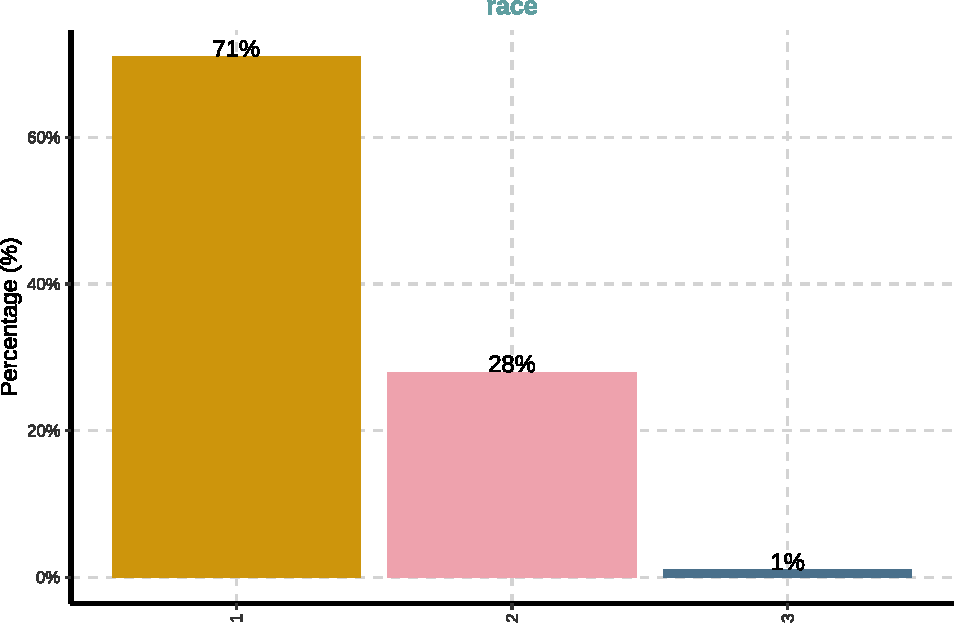
\includegraphics{notebook_panel_data_files/figure-latex/Exploratory data analysis-1.pdf}

\begin{verbatim}
## 
## [[2]]
\end{verbatim}

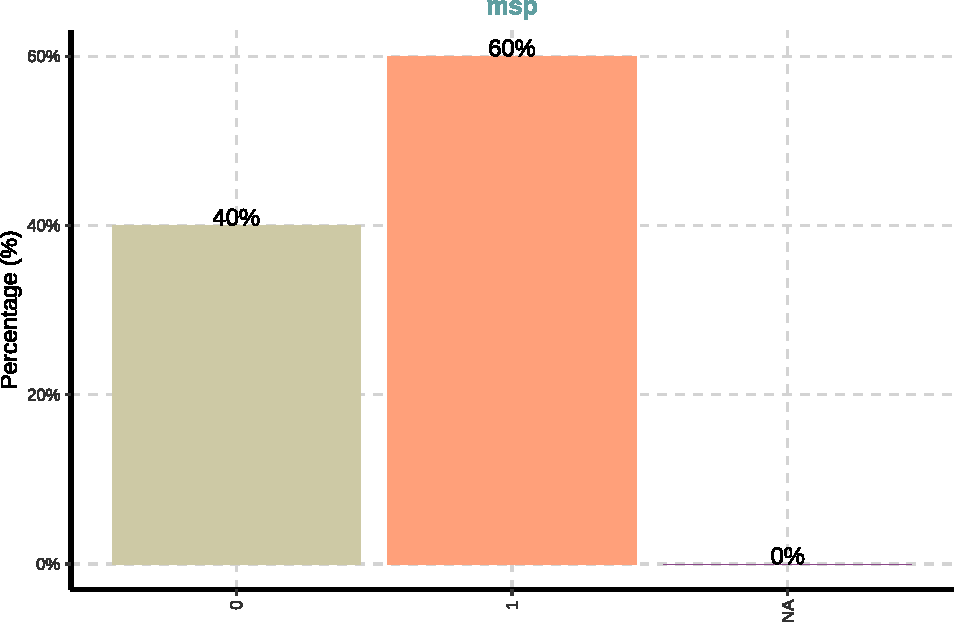
\includegraphics{notebook_panel_data_files/figure-latex/Exploratory data analysis-2.pdf}

\begin{verbatim}
## 
## [[3]]
\end{verbatim}

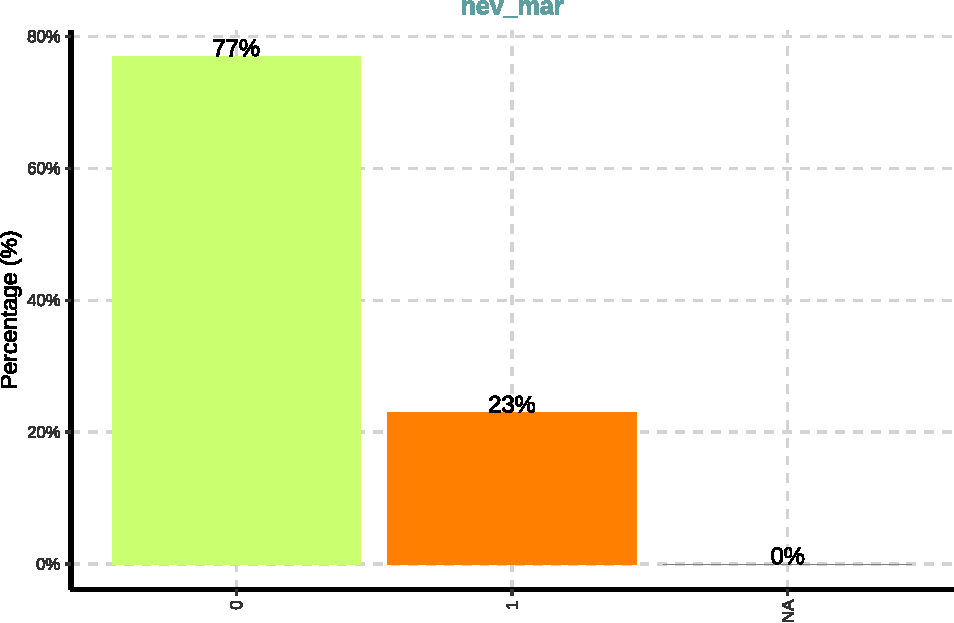
\includegraphics{notebook_panel_data_files/figure-latex/Exploratory data analysis-3.pdf}

\begin{verbatim}
## 
## [[4]]
\end{verbatim}

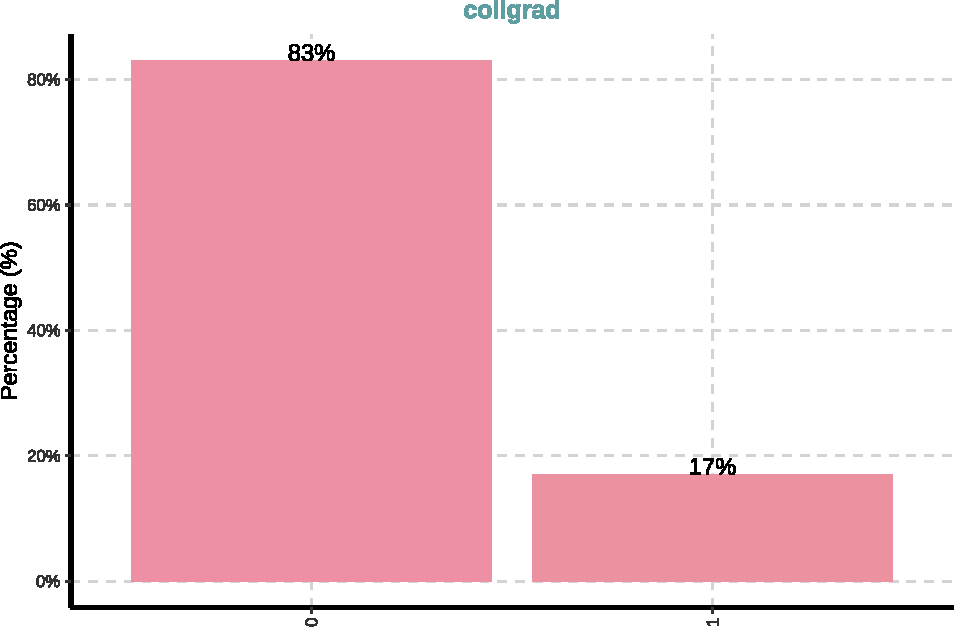
\includegraphics{notebook_panel_data_files/figure-latex/Exploratory data analysis-4.pdf}

\begin{verbatim}
## 
## [[5]]
\end{verbatim}

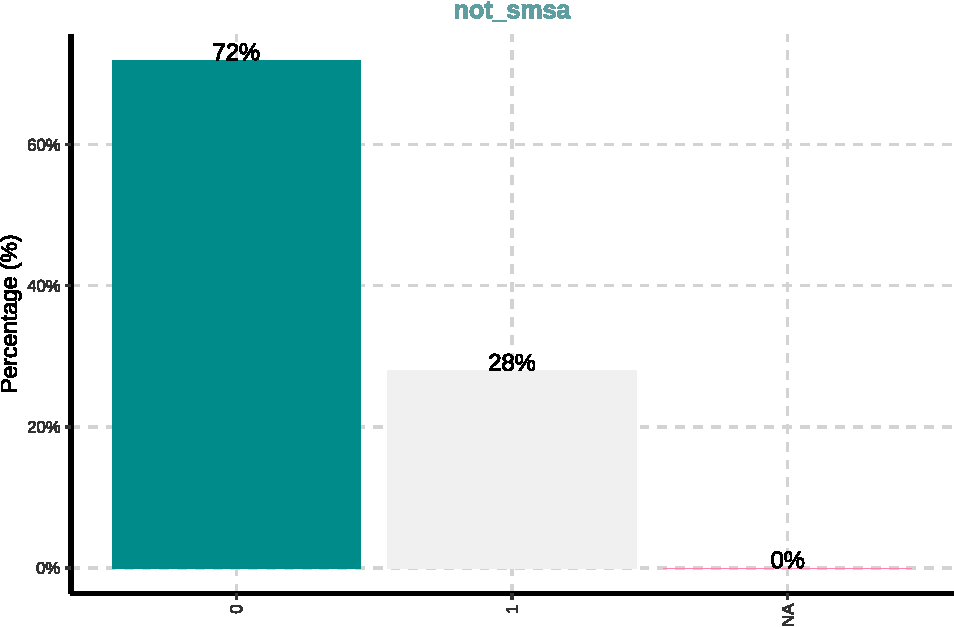
\includegraphics{notebook_panel_data_files/figure-latex/Exploratory data analysis-5.pdf}

\begin{verbatim}
## 
## [[6]]
\end{verbatim}

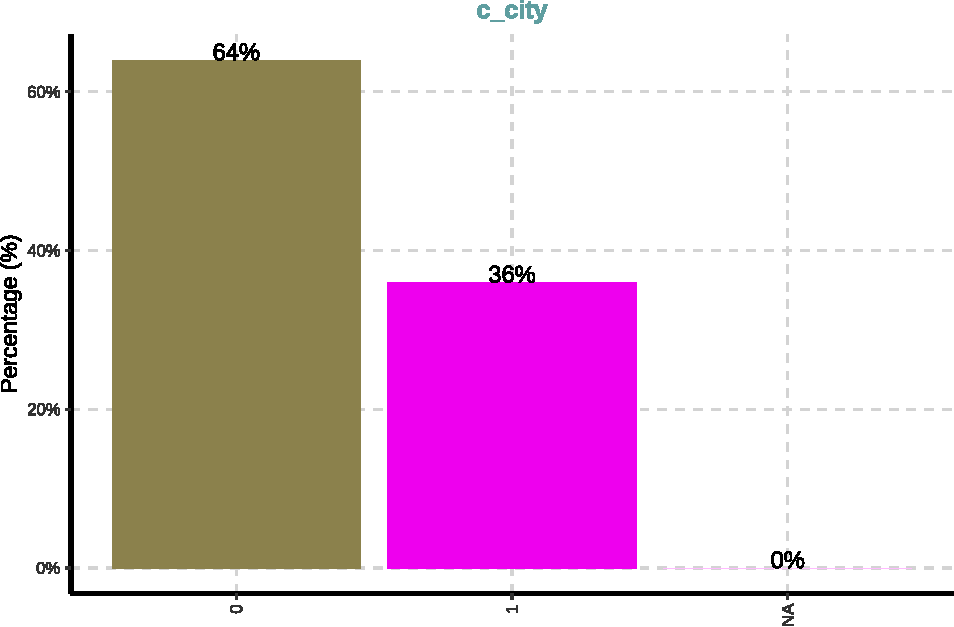
\includegraphics{notebook_panel_data_files/figure-latex/Exploratory data analysis-6.pdf}

\begin{verbatim}
## 
## [[7]]
\end{verbatim}

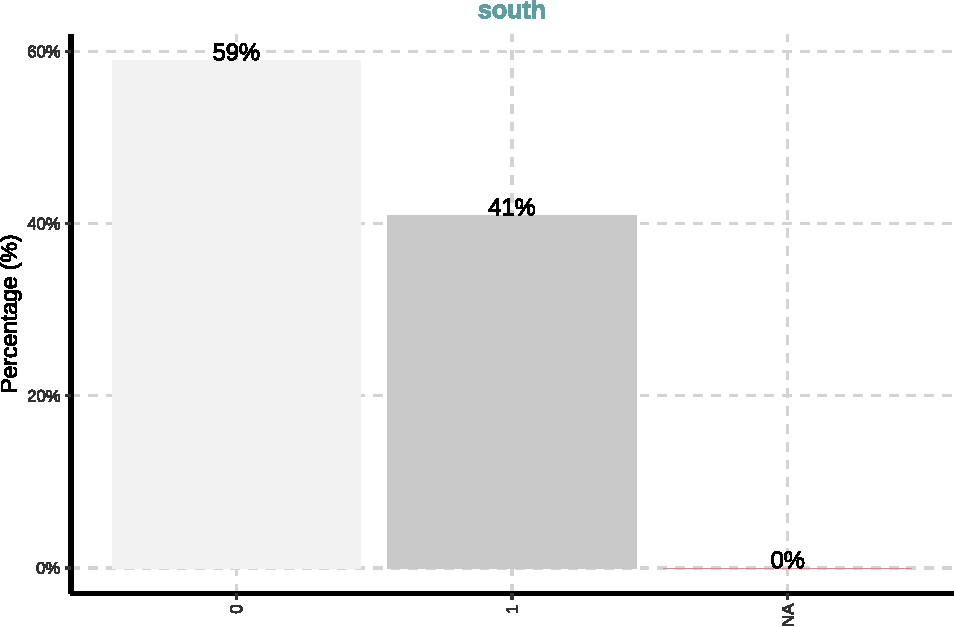
\includegraphics{notebook_panel_data_files/figure-latex/Exploratory data analysis-7.pdf}

\begin{verbatim}
## 
## [[8]]
\end{verbatim}

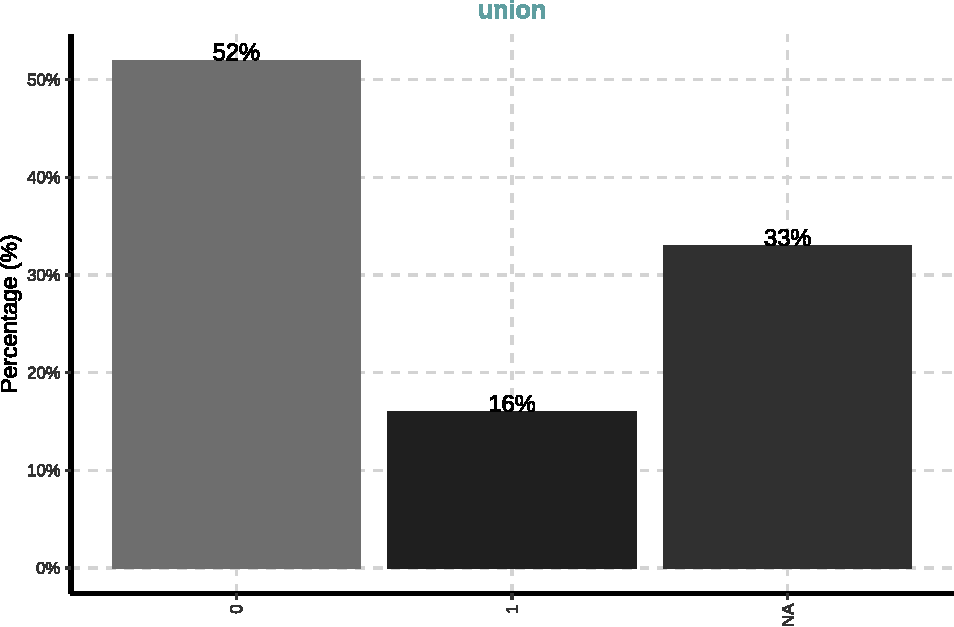
\includegraphics{notebook_panel_data_files/figure-latex/Exploratory data analysis-8.pdf}

\begin{verbatim}
## $`0`
\end{verbatim}

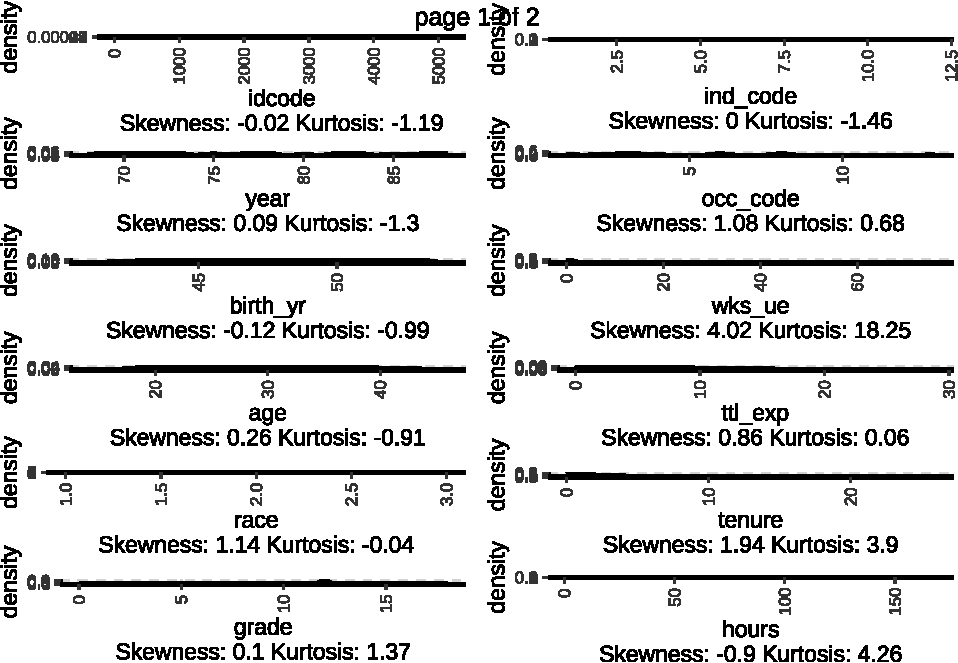
\includegraphics{notebook_panel_data_files/figure-latex/Exploratory data analysis-9.pdf}
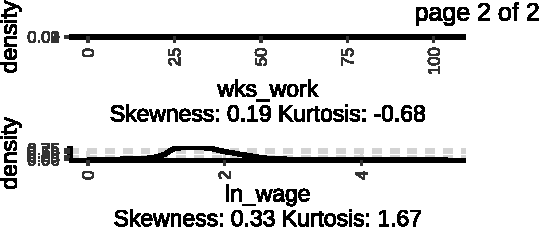
\includegraphics{notebook_panel_data_files/figure-latex/Exploratory data analysis-10.pdf}

\hypertarget{missing-values}{%
\subsection{MISSING VALUES}\label{missing-values}}

\begin{Shaded}
\begin{Highlighting}[]
  \FunctionTok{vis\_dat}\NormalTok{(nlswork)}
\end{Highlighting}
\end{Shaded}

\begin{verbatim}
## Warning: `gather_()` was deprecated in tidyr 1.2.0.
## i Please use `gather()` instead.
## i The deprecated feature was likely used in the visdat package.
##   Please report the issue at <]8;;https://github.com/ropensci/visdat/issueshttps://github.com/ropensci/visdat/issues]8;;>.
\end{verbatim}

\includegraphics{notebook_panel_data_files/figure-latex/Missing values-1.pdf}

\begin{Shaded}
\begin{Highlighting}[]
\CommentTok{\# vis\_miss(nlswork) \# ALTERNATIVE}

  \FunctionTok{gg\_miss\_upset}\NormalTok{(nlswork)}
\end{Highlighting}
\end{Shaded}

\includegraphics{notebook_panel_data_files/figure-latex/Missing values-2.pdf}

\hypertarget{add-a-dataframe}{%
\subsection{Add a dataframe}\label{add-a-dataframe}}

\hypertarget{export-output}{%
\subsection{Export output}\label{export-output}}

\begin{Shaded}
\begin{Highlighting}[]
  \FunctionTok{stargazer}\NormalTok{(nls,}
            \AttributeTok{title =} \StringTok{"Summary statistics"}\NormalTok{,}
            \AttributeTok{label =} \StringTok{"tb:statistcis"}\NormalTok{,}
            \AttributeTok{table.placement =} \StringTok{"ht"}\NormalTok{,}
            \AttributeTok{header=}\ConstantTok{FALSE}\NormalTok{,}\AttributeTok{type=}\StringTok{"text"}\NormalTok{)}
\end{Highlighting}
\end{Shaded}

\begin{verbatim}
## 
## Summary statistics
## =================================================
## Statistic   N      Mean    St. Dev.   Min   Max  
## -------------------------------------------------
## idcode    28,534 2,601.284 1,487.359   1   5,159 
## year      28,534  77.959     6.384    68     88  
## birth_yr  28,534  48.085     3.013    41     54  
## age       28,510  29.045     6.701    14     46  
## race      28,534   1.303     0.482     1     3   
## msp       28,518   0.603     0.489     0     1   
## nev_mar   28,518   0.230     0.421     0     1   
## grade     28,532  12.533     2.324     0     18  
## collgrad  28,534   0.168     0.374     0     1   
## not_smsa  28,526   0.282     0.450     0     1   
## c_city    28,526   0.357     0.479     0     1   
## south     28,526   0.410     0.492     0     1   
## ind_code  28,193   7.693     2.994     1     12  
## occ_code  28,413   4.778     3.065     1     13  
## union     19,238   0.234     0.424     0     1   
## wks_ue    22,830   2.548     7.294     0     76  
## ttl_exp   28,534   6.215     4.652   0.000 28.885
## tenure    28,101   3.124     3.751   0.000 25.917
## hours     28,467  36.560     9.870     1    168  
## wks_work  27,831  53.989    29.032     0    104  
## ln_wage   28,534   1.675     0.478   0.000 5.264 
## -------------------------------------------------
\end{verbatim}

\hypertarget{produce-a-graph}{%
\subsection{Produce a graph}\label{produce-a-graph}}

\hypertarget{save-the-graph}{%
\subsection{Save the graph}\label{save-the-graph}}

\hypertarget{tabulations-and-further-statistics}{%
\subsection{Tabulations and further
statistics}\label{tabulations-and-further-statistics}}

\begin{verbatim}
##  nlswork$race     n    percent
##             1 20180 0.70722647
##             2  8051 0.28215462
##             3   303 0.01061891
\end{verbatim}

\begin{verbatim}
## Frequencies  
## nlswork$year  
## Label: interview year  
## Type: Numeric  
## 
##                Freq   % Valid   % Valid Cum.   % Total   % Total Cum.
## ----------- ------- --------- -------------- --------- --------------
##          88    2272      7.96           7.96      7.96           7.96
##          77    2171      7.61          15.57      7.61          15.57
##          87    2164      7.58          23.15      7.58          23.15
##          75    2141      7.50          30.66      7.50          30.66
##          82    2085      7.31          37.97      7.31          37.97
##          85    2085      7.31          45.27      7.31          45.27
##          83    1987      6.96          52.24      6.96          52.24
##          73    1981      6.94          59.18      6.94          59.18
##          78    1964      6.88          66.06      6.88          66.06
##          71    1851      6.49          72.55      6.49          72.55
##          80    1847      6.47          79.02      6.47          79.02
##          72    1693      5.93          84.95      5.93          84.95
##          70    1686      5.91          90.86      5.91          90.86
##          68    1375      4.82          95.68      4.82          95.68
##          69    1232      4.32         100.00      4.32         100.00
##        <NA>       0                               0.00         100.00
##       Total   28534    100.00         100.00    100.00         100.00
\end{verbatim}

\begin{verbatim}
## Frequencies  
## nlswork$race  
## Label: 1=white, 2=black, 3=other  
## Type: Numeric  
## 
##                Freq   % Valid   % Valid Cum.   % Total   % Total Cum.
## ----------- ------- --------- -------------- --------- --------------
##           1   20180     70.72          70.72     70.72          70.72
##           2    8051     28.22          98.94     28.22          98.94
##           3     303      1.06         100.00      1.06         100.00
##        <NA>       0                               0.00         100.00
##       Total   28534    100.00         100.00    100.00         100.00
\end{verbatim}

\hypertarget{a-new-dataset-exclude-onservations-with-missing-information-in-a-subset-of-variables}{%
\section{A new dataset: exclude onservations with missing information in
a subset of
variables}\label{a-new-dataset-exclude-onservations-with-missing-information-in-a-subset-of-variables}}

\hypertarget{add-variable}{%
\subsection{Add variable}\label{add-variable}}

\hypertarget{plot-variables-means}{%
\subsection{Plot variables means}\label{plot-variables-means}}

\includegraphics{notebook_panel_data_files/figure-latex/Plot variables means-1.pdf}

\hypertarget{regression-analysis}{%
\section{Regression analysis}\label{regression-analysis}}

\begin{itemize}
\item
  \emph{Estimating a Mincerian Wage Equation}
\item
  \emph{POLS estimator with cluster-robust standard errors}
\end{itemize}

\hypertarget{q1}{%
\subsection{\texorpdfstring{\emph{Q1}}{Q1}}\label{q1}}

\hypertarget{pooled-ols-model}{%
\subsubsection{Pooled OLS model}\label{pooled-ols-model}}

\hypertarget{export-regression-output}{%
\subsection{Export regression output}\label{export-regression-output}}

\begin{verbatim}
## 
## Regression analysis
## =================================================
##                        OLS             panel     
##                                       linear     
##                        OLS            Pooled     
## -------------------------------------------------
## Union                0.113***        0.113***    
##                      (0.007)          (0.007)    
## Collage Graduate     0.351***        0.351***    
##                      (0.007)          (0.007)    
## Age                  0.022***        0.022***    
##                      (0.004)          (0.004)    
## Age sqrd.           -0.0003***      -0.0003***   
##                      (0.0001)        (0.0001)    
## Tenure               0.055***        0.055***    
##                      (0.002)          (0.002)    
## Tenure sqrd.        -0.002***        -0.002***   
##                      (0.0001)        (0.0001)    
## Not SMSA            -0.205***        -0.205***   
##                      (0.007)          (0.007)    
## South               -0.141***        -0.141***   
##                      (0.006)          (0.006)    
## City                -0.032***        -0.032***   
##                      (0.007)          (0.007)    
## N                     19,007          19,007     
## R2                    0.319            0.319     
## =================================================
## Notes:           Standard errors in parentheses.
\end{verbatim}

\begin{itemize}
\tightlist
\item
  \emph{SMSA}: Standard Metropolitan Statistical Area
\end{itemize}

\begin{Shaded}
\begin{Highlighting}[]
\CommentTok{\# ftable(c\_city) \# 1 if central city}
\end{Highlighting}
\end{Shaded}

\hypertarget{clustered-standard-errors}{%
\section{CLUSTERED Standard-errors}\label{clustered-standard-errors}}

\begin{Shaded}
\begin{Highlighting}[]
\NormalTok{  pols\_robust }\OtherTok{\textless{}{-}} \FunctionTok{coeftest}\NormalTok{(pols, }\ControlFlowTok{function}\NormalTok{(x) }\FunctionTok{vcovHC}\NormalTok{(x, }\AttributeTok{type =} \StringTok{\textquotesingle{}sss\textquotesingle{}}\NormalTok{)) }
  
  \FunctionTok{stargazer}\NormalTok{(pols,pols\_robust,}\AttributeTok{title =} \StringTok{"Regression analysis"}\NormalTok{, }
            \AttributeTok{model.numbers =} \ConstantTok{FALSE}\NormalTok{,}
            \AttributeTok{column.labels =} \FunctionTok{c}\NormalTok{(}\StringTok{"Pooled"}\NormalTok{,}\StringTok{"Pooled (cluster)"}\NormalTok{),}
            \AttributeTok{label =} \StringTok{"regressions"}\NormalTok{,}
            \AttributeTok{table.placement =} \StringTok{"!ht"}\NormalTok{,}
            \AttributeTok{notes.append =} \ConstantTok{FALSE}\NormalTok{,}
            \AttributeTok{notes.align=}\StringTok{"l"}\NormalTok{,}
            \AttributeTok{notes=}\StringTok{"Standard errors in parentheses."}\NormalTok{,}
            \AttributeTok{header =} \ConstantTok{FALSE}\NormalTok{,}
            \AttributeTok{no.space =} \ConstantTok{TRUE}\NormalTok{,}
            \AttributeTok{covariate.labels =} \FunctionTok{c}\NormalTok{(}\StringTok{"Union"}\NormalTok{,}\StringTok{"Collage graduate"}\NormalTok{,}\StringTok{"Age"}\NormalTok{,}\StringTok{"Age sqrd."}\NormalTok{,}
                                 \StringTok{"Tenure"}\NormalTok{,}\StringTok{"Tenure sqrd."}\NormalTok{,}\StringTok{"Not SMSA"}\NormalTok{,}\StringTok{"South"}\NormalTok{,}\StringTok{"City"}\NormalTok{),}
            \AttributeTok{omit =} \FunctionTok{c}\NormalTok{(}\StringTok{"Constant"}\NormalTok{),}
            \AttributeTok{omit.stat =} \FunctionTok{c}\NormalTok{(}\StringTok{"adj.rsq"}\NormalTok{,}\StringTok{"f"}\NormalTok{,}\StringTok{"ser"}\NormalTok{),}
            \AttributeTok{digits =} \DecValTok{6}\NormalTok{,}
            \AttributeTok{digits.extra =} \DecValTok{7}\NormalTok{,}
            \AttributeTok{omit.yes.no =} \FunctionTok{c}\NormalTok{(}\StringTok{"Constant"}\NormalTok{,}\StringTok{""}\NormalTok{),}
            \AttributeTok{dep.var.caption=}\StringTok{""}\NormalTok{,}
            \AttributeTok{dep.var.labels.include =} \ConstantTok{FALSE}\NormalTok{,}
            \AttributeTok{style =} \StringTok{"qje"}\NormalTok{,}
            \AttributeTok{type=}\StringTok{"text"}\NormalTok{)}
\end{Highlighting}
\end{Shaded}

\begin{verbatim}
## 
## Regression analysis
## =================================================
##                       panel        coefficient   
##                      linear            test      
##                      Pooled      Pooled (cluster)
## -------------------------------------------------
## Union              0.112774***     0.112774***   
##                    (0.006774)       (0.011731)   
## Collage graduate   0.350946***     0.350946***   
##                    (0.007149)       (0.014112)   
## Age                0.022481***     0.022481***   
##                    (0.004249)       (0.005373)   
## Age sqrd.         -0.000306***     -0.000306***  
##                    (0.000068)       (0.000088)   
## Tenure             0.054787***     0.054787***   
##                    (0.001944)       (0.002743)   
## Tenure sqrd.      -0.001540***     -0.001540***  
##                    (0.000125)       (0.000180)   
## Not SMSA          -0.205457***     -0.205457***  
##                    (0.007120)       (0.013137)   
## South             -0.140589***     -0.140589***  
##                    (0.005850)       (0.010964)   
## City              -0.031543***     -0.031543***  
##                    (0.006683)       (0.011691)   
## N                    19,007                      
## R2                  0.319459                     
## =================================================
## Notes:           Standard errors in parentheses.
\end{verbatim}

\hypertarget{q2}{%
\subsection{\texorpdfstring{\emph{Q2}}{Q2}}\label{q2}}

\hypertarget{random-effects-estimator-re}{%
\subsubsection{\texorpdfstring{\emph{Random effects estimator
(RE)}}{Random effects estimator (RE)}}\label{random-effects-estimator-re}}

\begin{itemize}
\tightlist
\item
  SEE THE DISCUSSION HERE for the comparison between R and Stata
\end{itemize}

\hypertarget{httpsstats.stackexchange.comquestions421374different-results-from-random-effects-plm-r-and-xtreg-stata}{%
\section{\texorpdfstring{\url{https://stats.stackexchange.com/questions/421374/different-results-from-random-effects-plm-r-and-xtreg-stata}}{https://stats.stackexchange.com/questions/421374/different-results-from-random-effects-plm-r-and-xtreg-stata}}\label{httpsstats.stackexchange.comquestions421374different-results-from-random-effects-plm-r-and-xtreg-stata}}

\begin{itemize}
\tightlist
\item
  R and Stata treat differently unbalanced panels
\end{itemize}

\textbf{for a balanced panel we have}

\begin{Shaded}
\begin{Highlighting}[]
\NormalTok{  nlswork\_balanced }\OtherTok{\textless{}{-}} \FunctionTok{read\_dta}\NormalTok{(}\StringTok{"data/nlswork\_balanced.dta"}\NormalTok{)}
  
\NormalTok{  re\_balanced }\OtherTok{\textless{}{-}} \FunctionTok{plm}\NormalTok{(}\AttributeTok{data =}\NormalTok{ nlswork\_balanced, ln\_wage }\SpecialCharTok{\textasciitilde{}}\NormalTok{ union }\SpecialCharTok{+}
\NormalTok{                       collgrad }\SpecialCharTok{+}\NormalTok{age }\SpecialCharTok{+}\NormalTok{agesq }\SpecialCharTok{+}\NormalTok{tenure }\SpecialCharTok{+}\NormalTok{tensq }\SpecialCharTok{+}
\NormalTok{                       not\_smsa }\SpecialCharTok{+}\NormalTok{south }\SpecialCharTok{+}\NormalTok{c\_city, }\AttributeTok{model=}\StringTok{"random"}\NormalTok{,}
                     \AttributeTok{index=}\FunctionTok{c}\NormalTok{(}\StringTok{"idcode"}\NormalTok{, }\StringTok{"year"}\NormalTok{))}
      \FunctionTok{summary}\NormalTok{(re\_balanced)}
\end{Highlighting}
\end{Shaded}

\begin{verbatim}
## Oneway (individual) effect Random Effect Model 
##    (Swamy-Arora's transformation)
## 
## Call:
## plm(formula = ln_wage ~ union + collgrad + age + agesq + tenure + 
##     tensq + not_smsa + south + c_city, data = nlswork_balanced, 
##     model = "random", index = c("idcode", "year"))
## 
## Balanced Panel: n = 53, T = 12, N = 636
## 
## Effects:
##                   var std.dev share
## idiosyncratic 0.03698 0.19230 0.319
## individual    0.07902 0.28110 0.681
## theta: 0.8063
## 
## Residuals:
##      Min.   1st Qu.    Median   3rd Qu.      Max. 
## -0.904519 -0.104813  0.015673  0.114854  0.658580 
## 
## Coefficients:
##                Estimate  Std. Error z-value  Pr(>|z|)    
## (Intercept)  1.05650211  0.20514289  5.1501 2.604e-07 ***
## union        0.06087668  0.02949229  2.0642 0.0390030 *  
## collgrad     0.20128253  0.17651938  1.1403 0.2541673    
## age          0.04592525  0.01334703  3.4409 0.0005799 ***
## agesq       -0.00051693  0.00020986 -2.4632 0.0137701 *  
## tenure       0.00332254  0.00616575  0.5389 0.5899766    
## tensq        0.00011290  0.00028483  0.3964 0.6918193    
## not_smsa    -0.29590935  0.07567198 -3.9104 9.214e-05 ***
## south       -0.06346941  0.06258349 -1.0142 0.3105084    
## c_city       0.00068168  0.03609511  0.0189 0.9849322    
## ---
## Signif. codes:  0 '***' 0.001 '**' 0.01 '*' 0.05 '.' 0.1 ' ' 1
## 
## Total Sum of Squares:    32.65
## Residual Sum of Squares: 23.689
## R-Squared:      0.27447
## Adj. R-Squared: 0.26404
## Chisq: 236.819 on 9 DF, p-value: < 2.22e-16
\end{verbatim}

\begin{Shaded}
\begin{Highlighting}[]
\NormalTok{  re }\OtherTok{\textless{}{-}} \FunctionTok{plm}\NormalTok{(}\AttributeTok{data =}\NormalTok{ nlswork\_clean, ln\_wage }\SpecialCharTok{\textasciitilde{}}\NormalTok{ union }\SpecialCharTok{+}
\NormalTok{              collgrad }\SpecialCharTok{+}\NormalTok{age }\SpecialCharTok{+}\NormalTok{agesq }\SpecialCharTok{+}\NormalTok{tenure }\SpecialCharTok{+}\NormalTok{tensq }\SpecialCharTok{+}
\NormalTok{              not\_smsa }\SpecialCharTok{+}\NormalTok{south }\SpecialCharTok{+}\NormalTok{c\_city, }\AttributeTok{model=}\StringTok{"random"}\NormalTok{,}
            \AttributeTok{index=}\FunctionTok{c}\NormalTok{(}\StringTok{"idcode"}\NormalTok{, }\StringTok{"year"}\NormalTok{))}
      \CommentTok{\# summary(re)}

\NormalTok{  re\_robust }\OtherTok{\textless{}{-}} \FunctionTok{coeftest}\NormalTok{(re, }\ControlFlowTok{function}\NormalTok{(x) }\FunctionTok{vcovHC}\NormalTok{(x, }\AttributeTok{type =} \StringTok{\textquotesingle{}sss\textquotesingle{}}\NormalTok{))}
\end{Highlighting}
\end{Shaded}

\begin{Shaded}
\begin{Highlighting}[]
  \FunctionTok{stargazer}\NormalTok{(pols,pols\_robust,re,re\_robust,}\AttributeTok{title =} \StringTok{"Regression analysis"}\NormalTok{, }
            \AttributeTok{model.numbers =} \ConstantTok{FALSE}\NormalTok{,}
            \AttributeTok{column.labels =} \FunctionTok{c}\NormalTok{(}\StringTok{"Pooled"}\NormalTok{,}\StringTok{"Pooled (cluster)"}\NormalTok{,}\StringTok{"RE"}\NormalTok{,}\StringTok{"RE (cluster"}\NormalTok{),}
            \AttributeTok{label =} \StringTok{"regressions"}\NormalTok{,}
            \AttributeTok{table.placement =} \StringTok{"!ht"}\NormalTok{,}
            \AttributeTok{notes.append =} \ConstantTok{FALSE}\NormalTok{,}
            \AttributeTok{notes.align=}\StringTok{"l"}\NormalTok{,}
            \AttributeTok{notes=}\StringTok{"Standard errors in parentheses."}\NormalTok{,}
            \AttributeTok{header =} \ConstantTok{FALSE}\NormalTok{,}
            \AttributeTok{no.space =} \ConstantTok{TRUE}\NormalTok{,}
            \AttributeTok{covariate.labels =} \FunctionTok{c}\NormalTok{(}\StringTok{"Union"}\NormalTok{,}\StringTok{"College Graduate"}\NormalTok{,}\StringTok{"Age"}\NormalTok{,}\StringTok{"Age sqrd."}\NormalTok{,}
                                 \StringTok{"Tenure"}\NormalTok{,}\StringTok{"Tenure sqrd."}\NormalTok{,}\StringTok{"Not SMSA"}\NormalTok{,}\StringTok{"South"}\NormalTok{,}\StringTok{"City"}\NormalTok{),}
            \AttributeTok{omit =} \FunctionTok{c}\NormalTok{(}\StringTok{"Constant"}\NormalTok{),}
            \AttributeTok{omit.stat =} \FunctionTok{c}\NormalTok{(}\StringTok{"adj.rsq"}\NormalTok{,}\StringTok{"f"}\NormalTok{,}\StringTok{"ser"}\NormalTok{),}
            \AttributeTok{digits =} \DecValTok{3}\NormalTok{,}
            \AttributeTok{digits.extra =} \DecValTok{5}\NormalTok{,}
            \AttributeTok{omit.yes.no =} \FunctionTok{c}\NormalTok{(}\StringTok{"Constant"}\NormalTok{,}\StringTok{""}\NormalTok{),}
            \AttributeTok{dep.var.caption=}\StringTok{""}\NormalTok{,}
            \AttributeTok{dep.var.labels.include =} \ConstantTok{FALSE}\NormalTok{,}
            \AttributeTok{style =} \StringTok{"qje"}\NormalTok{,}
            \AttributeTok{type=}\StringTok{"text"}\NormalTok{)}
\end{Highlighting}
\end{Shaded}

\begin{verbatim}
## 
## Regression analysis
## ===================================================================
##                    panel      coefficient      panel    coefficient
##                    linear         test         linear      test    
##                    Pooled   Pooled (cluster)     RE     RE (cluster
## -------------------------------------------------------------------
## Union             0.113***      0.113***      0.104***   0.104***  
##                   (0.007)       (0.012)       (0.006)     (0.009)  
## College Graduate  0.351***      0.351***      0.369***   0.369***  
##                   (0.007)       (0.014)       (0.012)     (0.013)  
## Age               0.022***      0.022***      0.023***   0.023***  
##                   (0.004)       (0.005)       (0.003)     (0.005)  
## Age sqrd.        -0.0003***    -0.0003***    -0.0002*** -0.0002*** 
##                   (0.0001)      (0.0001)      (0.0001)   (0.0001)  
## Tenure            0.055***      0.055***      0.041***   0.041***  
##                   (0.002)       (0.003)       (0.002)     (0.002)  
## Tenure sqrd.     -0.002***     -0.002***     -0.001***   -0.001*** 
##                   (0.0001)      (0.0002)      (0.0001)   (0.0001)  
## Not SMSA         -0.205***     -0.205***     -0.151***   -0.151*** 
##                   (0.007)       (0.013)       (0.009)     (0.012)  
## South            -0.141***     -0.141***     -0.112***   -0.112*** 
##                   (0.006)       (0.011)       (0.008)     (0.011)  
## City             -0.032***     -0.032***       0.0004     0.0004   
##                   (0.007)       (0.012)       (0.007)     (0.010)  
## N                  19,007                      19,007              
## R2                 0.319                       0.349               
## ===================================================================
## Notes:           Standard errors in parentheses.
\end{verbatim}

\begin{Shaded}
\begin{Highlighting}[]
  \FunctionTok{stargazer}\NormalTok{(pols,pols\_robust,re,re\_robust,}\AttributeTok{title =} \StringTok{"Regression analysis"}\NormalTok{, }
            \AttributeTok{model.numbers =} \ConstantTok{FALSE}\NormalTok{,}
            \AttributeTok{column.labels =} \FunctionTok{c}\NormalTok{(}\StringTok{"Pooled"}\NormalTok{,}\StringTok{"Pooled (cluster)"}\NormalTok{,}\StringTok{"RE"}\NormalTok{,}\StringTok{"RE (cluster"}\NormalTok{),}
            \AttributeTok{label =} \StringTok{"regressions"}\NormalTok{,}
            \AttributeTok{table.placement =} \StringTok{"!ht"}\NormalTok{,}
            \AttributeTok{notes.append =} \ConstantTok{FALSE}\NormalTok{,}
            \AttributeTok{notes.align=}\StringTok{"l"}\NormalTok{,}
            \AttributeTok{notes=}\StringTok{"Standard errors in parentheses."}\NormalTok{,}
            \AttributeTok{header =} \ConstantTok{FALSE}\NormalTok{,}
            \AttributeTok{no.space =} \ConstantTok{TRUE}\NormalTok{,}
            \AttributeTok{covariate.labels =} \FunctionTok{c}\NormalTok{(}\StringTok{"Union"}\NormalTok{,}\StringTok{"College Graduate"}\NormalTok{,}\StringTok{"Age"}\NormalTok{,}\StringTok{"Age sqrd."}\NormalTok{,}
                                 \StringTok{"Tenure"}\NormalTok{,}\StringTok{"Tenure sqrd."}\NormalTok{,}\StringTok{"Not SMSA"}\NormalTok{,}\StringTok{"South"}\NormalTok{,}\StringTok{"City"}\NormalTok{),}
            \AttributeTok{omit =} \FunctionTok{c}\NormalTok{(}\StringTok{"Constant"}\NormalTok{),}
            \AttributeTok{omit.stat =} \FunctionTok{c}\NormalTok{(}\StringTok{"adj.rsq"}\NormalTok{,}\StringTok{"f"}\NormalTok{,}\StringTok{"ser"}\NormalTok{),}
            \AttributeTok{digits =} \DecValTok{3}\NormalTok{,}
            \AttributeTok{digits.extra =} \DecValTok{5}\NormalTok{,}
            \AttributeTok{omit.yes.no =} \FunctionTok{c}\NormalTok{(}\StringTok{"Constant"}\NormalTok{,}\StringTok{""}\NormalTok{),}
            \AttributeTok{dep.var.caption=}\StringTok{""}\NormalTok{,}
            \AttributeTok{dep.var.labels.include =} \ConstantTok{FALSE}\NormalTok{,}
            \AttributeTok{style =} \StringTok{"qje"}\NormalTok{,}
            \AttributeTok{type=}\StringTok{"text"}\NormalTok{)}
\end{Highlighting}
\end{Shaded}

\begin{verbatim}
## 
## Regression analysis
## ===================================================================
##                    panel      coefficient      panel    coefficient
##                    linear         test         linear      test    
##                    Pooled   Pooled (cluster)     RE     RE (cluster
## -------------------------------------------------------------------
## Union             0.113***      0.113***      0.104***   0.104***  
##                   (0.007)       (0.012)       (0.006)     (0.009)  
## College Graduate  0.351***      0.351***      0.369***   0.369***  
##                   (0.007)       (0.014)       (0.012)     (0.013)  
## Age               0.022***      0.022***      0.023***   0.023***  
##                   (0.004)       (0.005)       (0.003)     (0.005)  
## Age sqrd.        -0.0003***    -0.0003***    -0.0002*** -0.0002*** 
##                   (0.0001)      (0.0001)      (0.0001)   (0.0001)  
## Tenure            0.055***      0.055***      0.041***   0.041***  
##                   (0.002)       (0.003)       (0.002)     (0.002)  
## Tenure sqrd.     -0.002***     -0.002***     -0.001***   -0.001*** 
##                   (0.0001)      (0.0002)      (0.0001)   (0.0001)  
## Not SMSA         -0.205***     -0.205***     -0.151***   -0.151*** 
##                   (0.007)       (0.013)       (0.009)     (0.012)  
## South            -0.141***     -0.141***     -0.112***   -0.112*** 
##                   (0.006)       (0.011)       (0.008)     (0.011)  
## City             -0.032***     -0.032***       0.0004     0.0004   
##                   (0.007)       (0.012)       (0.007)     (0.010)  
## N                  19,007                      19,007              
## R2                 0.319                       0.349               
## ===================================================================
## Notes:           Standard errors in parentheses.
\end{verbatim}

\hypertarget{lm-test-for-the-presence-of-unobserved-effects}{%
\subsection{LM test for the presence of unobserved
effects}\label{lm-test-for-the-presence-of-unobserved-effects}}

\begin{Shaded}
\begin{Highlighting}[]
  \FunctionTok{plmtest}\NormalTok{(pols, }\AttributeTok{type=}\FunctionTok{c}\NormalTok{(}\StringTok{"bp"}\NormalTok{))}
\end{Highlighting}
\end{Shaded}

\begin{verbatim}
## 
##  Lagrange Multiplier Test - (Breusch-Pagan)
## 
## data:  ln_wage ~ union + collgrad + age + agesq + tenure + tensq + not_smsa +  ...
## chisq = 14041, df = 1, p-value < 2.2e-16
## alternative hypothesis: significant effects
\end{verbatim}

\begin{Shaded}
\begin{Highlighting}[]
  \FunctionTok{kable}\NormalTok{(}\FunctionTok{tidy}\NormalTok{(}\FunctionTok{plmtest}\NormalTok{(pols, }\AttributeTok{type=}\FunctionTok{c}\NormalTok{(}\StringTok{"bp"}\NormalTok{))), }\AttributeTok{format =} \StringTok{"simple"}\NormalTok{,}\AttributeTok{caption=}
          \StringTok{"LM test for the presence of unobserved effects"}\NormalTok{)}
\end{Highlighting}
\end{Shaded}

\begin{longtable}[]{@{}rrrll@{}}
\caption{LM test for the presence of unobserved effects}\tabularnewline
\toprule()
statistic & p.value & parameter & method & alternative \\
\midrule()
\endfirsthead
\toprule()
statistic & p.value & parameter & method & alternative \\
\midrule()
\endhead
14041.19 & 0 & 1 & Lagrange Multiplier Test - (Breusch-Pagan) &
significant effects \\
\bottomrule()
\end{longtable}

\hypertarget{fixed-effects-estimator-fe}{%
\subsection{Fixed effects estimator
(FE)}\label{fixed-effects-estimator-fe}}

\begin{Shaded}
\begin{Highlighting}[]
\CommentTok{\# //Final slide 32}
\CommentTok{\# }
\CommentTok{\# *Q3*}
\CommentTok{\#}

\NormalTok{  fe }\OtherTok{\textless{}{-}} \FunctionTok{plm}\NormalTok{(}\AttributeTok{data =}\NormalTok{ nlswork\_clean, ln\_wage }\SpecialCharTok{\textasciitilde{}}\NormalTok{ union }\SpecialCharTok{+}
\NormalTok{              collgrad }\SpecialCharTok{+}\NormalTok{age }\SpecialCharTok{+}\NormalTok{agesq }\SpecialCharTok{+}\NormalTok{tenure }\SpecialCharTok{+}\NormalTok{tensq }\SpecialCharTok{+}
\NormalTok{              not\_smsa }\SpecialCharTok{+}\NormalTok{south }\SpecialCharTok{+}\NormalTok{c\_city, }\AttributeTok{model=}\StringTok{"within"}\NormalTok{, }\AttributeTok{index=}\FunctionTok{c}\NormalTok{(}\StringTok{"idcode"}\NormalTok{, }\StringTok{"year"}\NormalTok{))}
      
      \FunctionTok{summary}\NormalTok{(fe)}
\end{Highlighting}
\end{Shaded}

\begin{verbatim}
## Oneway (individual) effect Within Model
## 
## Call:
## plm(formula = ln_wage ~ union + collgrad + age + agesq + tenure + 
##     tensq + not_smsa + south + c_city, data = nlswork_clean, 
##     model = "within", index = c("idcode", "year"))
## 
## Unbalanced Panel: n = 4134, T = 1-12, N = 19007
## 
## Residuals:
##     Min.  1st Qu.   Median  3rd Qu.     Max. 
## -1.88027 -0.10216  0.00000  0.10774  2.80710 
## 
## Coefficients:
##             Estimate  Std. Error  t-value  Pr(>|t|)    
## union     9.3877e-02  6.9662e-03  13.4761 < 2.2e-16 ***
## age       2.4259e-02  3.4467e-03   7.0383 2.031e-12 ***
## agesq    -2.2618e-04  5.5316e-05  -4.0890 4.356e-05 ***
## tenure    3.2966e-02  1.6465e-03  20.0218 < 2.2e-16 ***
## tensq    -1.1002e-03  1.0291e-04 -10.6916 < 2.2e-16 ***
## not_smsa -9.3105e-02  1.2970e-02  -7.1787 7.372e-13 ***
## south    -6.3222e-02  1.3279e-02  -4.7611 1.944e-06 ***
## c_city    1.1409e-02  8.8964e-03   1.2824    0.1997    
## ---
## Signif. codes:  0 '***' 0.001 '**' 0.01 '*' 0.05 '.' 0.1 ' ' 1
## 
## Total Sum of Squares:    1119.5
## Residual Sum of Squares: 962.69
## R-Squared:      0.14005
## Adj. R-Squared: -0.099505
## F-statistic: 302.62 on 8 and 14865 DF, p-value: < 2.22e-16
\end{verbatim}

\begin{Shaded}
\begin{Highlighting}[]
  \FunctionTok{stargazer}\NormalTok{(pols,re,fe,}\AttributeTok{title =} \StringTok{"Regression analysis"}\NormalTok{, }
            \AttributeTok{model.numbers =} \ConstantTok{FALSE}\NormalTok{,}
            \AttributeTok{column.labels =} \FunctionTok{c}\NormalTok{(}\StringTok{"Pooled"}\NormalTok{,}\StringTok{"RE"}\NormalTok{,}\StringTok{"FE"}\NormalTok{),}
            \AttributeTok{label =} \StringTok{"regressions"}\NormalTok{,}
            \AttributeTok{table.placement =} \StringTok{"!ht"}\NormalTok{,}
            \AttributeTok{notes.append =} \ConstantTok{FALSE}\NormalTok{,}
            \AttributeTok{notes.align=}\StringTok{"l"}\NormalTok{,}
            \AttributeTok{notes=}\StringTok{"Standard errors in parentheses."}\NormalTok{,}
            \AttributeTok{header =} \ConstantTok{FALSE}\NormalTok{,}
            \AttributeTok{no.space =} \ConstantTok{TRUE}\NormalTok{,}
            \AttributeTok{covariate.labels =} \FunctionTok{c}\NormalTok{(}\StringTok{"Union"}\NormalTok{,}\StringTok{"College"}\NormalTok{,}\StringTok{"Age"}\NormalTok{,}\StringTok{"Age sqrd."}\NormalTok{,}\StringTok{"Tenure"}\NormalTok{,}
                                 \StringTok{"Tenure sqrd."}\NormalTok{,}\StringTok{"Not SMSA"}\NormalTok{,}\StringTok{"South"}\NormalTok{,}\StringTok{"City"}\NormalTok{),}
            \AttributeTok{omit =} \FunctionTok{c}\NormalTok{(}\StringTok{"Constant"}\NormalTok{),}
            \AttributeTok{omit.stat =} \FunctionTok{c}\NormalTok{(}\StringTok{"adj.rsq"}\NormalTok{,}\StringTok{"f"}\NormalTok{,}\StringTok{"ser"}\NormalTok{),}
            \AttributeTok{digits =} \DecValTok{6}\NormalTok{,}
            \AttributeTok{digits.extra =} \DecValTok{7}\NormalTok{,}
            \AttributeTok{omit.yes.no =} \FunctionTok{c}\NormalTok{(}\StringTok{"Constant"}\NormalTok{,}\StringTok{""}\NormalTok{),}
            \AttributeTok{dep.var.caption=}\StringTok{""}\NormalTok{,}
            \AttributeTok{dep.var.labels.include =} \ConstantTok{FALSE}\NormalTok{,}
            \AttributeTok{style =} \StringTok{"qje"}\NormalTok{,}
            \AttributeTok{type=}\StringTok{"text"}\NormalTok{)}
\end{Highlighting}
\end{Shaded}

\begin{verbatim}
## 
## Regression analysis
## ===================================================
##                 Pooled         RE           FE     
## Union        0.112774***  0.103677***  0.093877*** 
##               (0.006774)   (0.006447)   (0.006966) 
## College      0.350946***  0.369309***              
##               (0.007149)   (0.012344)              
## Age          0.022481***  0.023031***  0.024259*** 
##               (0.004249)   (0.003317)   (0.003447) 
## Age sqrd.    -0.000306*** -0.000249*** -0.000226***
##               (0.000068)   (0.000053)   (0.000055) 
## Tenure       0.054787***  0.040771***  0.032966*** 
##               (0.001944)   (0.001583)   (0.001646) 
## Tenure sqrd. -0.001540*** -0.001247*** -0.001100***
##               (0.000125)   (0.000100)   (0.000103) 
## Not SMSA     -0.205457*** -0.151136*** -0.093105***
##               (0.007120)   (0.009380)   (0.012970) 
## South        -0.140589*** -0.111567*** -0.063222***
##               (0.005850)   (0.008467)   (0.013279) 
## City         -0.031543***   0.000397     0.011409  
##               (0.006683)   (0.007492)   (0.008896) 
## N               19,007       19,007       19,007   
## R2             0.319459     0.349029     0.140054  
## ===================================================
## Notes:       Standard errors in parentheses.
\end{verbatim}

\begin{Shaded}
\begin{Highlighting}[]
\CommentTok{\# Testing for fixed effects, null: OLS better than fixed}
\CommentTok{\# \textquotesingle{}F test for individual effects\textquotesingle{} \textless{}\textless{}==\textgreater{}\textgreater{} \textquotesingle{}F test that all u\_i=0\textquotesingle{}}

\NormalTok{  ols\_0 }\OtherTok{\textless{}{-}} \FunctionTok{lm}\NormalTok{(}\AttributeTok{data =}\NormalTok{ nlswork\_clean, ln\_wage }\SpecialCharTok{\textasciitilde{}}\NormalTok{ union }\SpecialCharTok{+}
\NormalTok{                age }\SpecialCharTok{+}\NormalTok{agesq }\SpecialCharTok{+}\NormalTok{tenure }\SpecialCharTok{+}\NormalTok{tensq }\SpecialCharTok{+}
\NormalTok{                not\_smsa }\SpecialCharTok{+}\NormalTok{south }\SpecialCharTok{+}\NormalTok{c\_city)}
      \FunctionTok{summary}\NormalTok{(ols\_0)}
\end{Highlighting}
\end{Shaded}

\begin{verbatim}
## 
## Call:
## lm(formula = ln_wage ~ union + age + agesq + tenure + tensq + 
##     not_smsa + south + c_city, data = nlswork_clean)
## 
## Residuals:
##     Min      1Q  Median      3Q     Max 
## -1.7497 -0.2508 -0.0182  0.2379  3.4100 
## 
## Coefficients:
##               Estimate Std. Error t value Pr(>|t|)    
## (Intercept)  1.008e+00  6.821e-02  14.776  < 2e-16 ***
## union        1.294e-01  7.181e-03  18.026  < 2e-16 ***
## age          3.929e-02  4.495e-03   8.740  < 2e-16 ***
## agesq       -5.387e-04  7.175e-05  -7.509 6.24e-14 ***
## tenure       5.806e-02  2.062e-03  28.158  < 2e-16 ***
## tensq       -1.699e-03  1.331e-04 -12.765  < 2e-16 ***
## not_smsa    -2.311e-01  7.538e-03 -30.657  < 2e-16 ***
## south       -1.475e-01  6.208e-03 -23.762  < 2e-16 ***
## c_city      -3.451e-02  7.094e-03  -4.864 1.16e-06 ***
## ---
## Signif. codes:  0 '***' 0.001 '**' 0.01 '*' 0.05 '.' 0.1 ' ' 1
## 
## Residual standard error: 0.4091 on 18998 degrees of freedom
## Multiple R-squared:  0.2331, Adjusted R-squared:  0.2328 
## F-statistic: 721.9 on 8 and 18998 DF,  p-value: < 2.2e-16
\end{verbatim}

\begin{Shaded}
\begin{Highlighting}[]
  \FunctionTok{pFtest}\NormalTok{(fe, ols\_0)}
\end{Highlighting}
\end{Shaded}

\begin{verbatim}
## 
##  F test for individual effects
## 
## data:  ln_wage ~ union + collgrad + age + agesq + tenure + tensq + not_smsa +  ...
## F = 8.2833, df1 = 4133, df2 = 14865, p-value < 2.2e-16
## alternative hypothesis: significant effects
\end{verbatim}

\begin{Shaded}
\begin{Highlighting}[]
\CommentTok{\# generate fixed{-}effects}

\CommentTok{\# nlswork\_clean$specific\_effects \textless{}{-} fixef(fe)}

\CommentTok{\# *Q3.1*}

\NormalTok{  fe\_robust }\OtherTok{\textless{}{-}} \FunctionTok{coeftest}\NormalTok{(fe, }\ControlFlowTok{function}\NormalTok{(x) }\FunctionTok{vcovHC}\NormalTok{(x, }\AttributeTok{type =} \StringTok{\textquotesingle{}sss\textquotesingle{}}\NormalTok{)) }

  \FunctionTok{stargazer}\NormalTok{(ols\_0,fe,fe\_robust,}\AttributeTok{title =} \StringTok{"Regression analysis"}\NormalTok{, }
            \AttributeTok{model.numbers =} \ConstantTok{FALSE}\NormalTok{,}
            \AttributeTok{column.labels =} \FunctionTok{c}\NormalTok{(}\StringTok{"OLS"}\NormalTok{,}\StringTok{"FE"}\NormalTok{,}\StringTok{"FE (cluster)"}\NormalTok{),}
            \AttributeTok{label =} \StringTok{"regressions"}\NormalTok{,}
            \AttributeTok{table.placement =} \StringTok{"!ht"}\NormalTok{,}
            \AttributeTok{notes.append =} \ConstantTok{FALSE}\NormalTok{,}
            \AttributeTok{notes.align=}\StringTok{"l"}\NormalTok{,}
            \AttributeTok{notes=}\StringTok{"Standard errors in parentheses."}\NormalTok{,}
            \AttributeTok{header =} \ConstantTok{FALSE}\NormalTok{,}
            \AttributeTok{no.space =} \ConstantTok{TRUE}\NormalTok{,}
            \AttributeTok{covariate.labels =} \FunctionTok{c}\NormalTok{(}\StringTok{"Union"}\NormalTok{,}\StringTok{"Age"}\NormalTok{,}\StringTok{"Age sqrd."}\NormalTok{,}\StringTok{"Tenure"}\NormalTok{,}
                                 \StringTok{"Tenure sqrd."}\NormalTok{,}\StringTok{"Not SMSA"}\NormalTok{,}\StringTok{"South"}\NormalTok{,}\StringTok{"City"}\NormalTok{),}
            \AttributeTok{omit =} \FunctionTok{c}\NormalTok{(}\StringTok{"Constant"}\NormalTok{),}
            \AttributeTok{omit.stat =} \FunctionTok{c}\NormalTok{(}\StringTok{"adj.rsq"}\NormalTok{,}\StringTok{"f"}\NormalTok{,}\StringTok{"ser"}\NormalTok{),}
            \AttributeTok{digits =} \DecValTok{6}\NormalTok{,}
            \AttributeTok{digits.extra =} \DecValTok{7}\NormalTok{,}
            \AttributeTok{omit.yes.no =} \FunctionTok{c}\NormalTok{(}\StringTok{"Constant"}\NormalTok{,}\StringTok{""}\NormalTok{),}
            \AttributeTok{dep.var.caption=}\StringTok{""}\NormalTok{,}
            \AttributeTok{dep.var.labels.include =} \ConstantTok{FALSE}\NormalTok{,}
            \AttributeTok{style =} \StringTok{"qje"}\NormalTok{,}
            \AttributeTok{type=}\StringTok{"text"}\NormalTok{)}
\end{Highlighting}
\end{Shaded}

\begin{verbatim}
## 
## Regression analysis
## ===================================================
##                  OLS         panel     coefficient 
##                              linear        test    
##                  OLS           FE      FE (cluster)
## ---------------------------------------------------
## Union        0.129446***  0.093877***  0.093877*** 
##               (0.007181)   (0.006966)   (0.009565) 
## Age          0.039289***  0.024259***  0.024259*** 
##               (0.004495)   (0.003447)   (0.005008) 
## Age sqrd.    -0.000539*** -0.000226*** -0.000226***
##               (0.000072)   (0.000055)   (0.000081) 
## Tenure       0.058063***  0.032966***  0.032966*** 
##               (0.002062)   (0.001646)   (0.002085) 
## Tenure sqrd. -0.001699*** -0.001100*** -0.001100***
##               (0.000133)   (0.000103)   (0.000126) 
## Not SMSA     -0.231095*** -0.093105*** -0.093105***
##               (0.007538)   (0.012970)   (0.019790) 
## South        -0.147518*** -0.063222*** -0.063222***
##               (0.006208)   (0.013279)   (0.021653) 
## City         -0.034506***   0.011409     0.011409  
##               (0.007094)   (0.008896)   (0.012605) 
## N               19,007       19,007                
## R2             0.233124     0.140054               
## ===================================================
## Notes:       Standard errors in parentheses.
\end{verbatim}

\begin{Shaded}
\begin{Highlighting}[]
\CommentTok{\# *Q3.2*}

  \FunctionTok{linearHypothesis}\NormalTok{(ols,}\FunctionTok{c}\NormalTok{(}\StringTok{"age=0"}\NormalTok{,}\StringTok{"agesq=0"}\NormalTok{))}
\end{Highlighting}
\end{Shaded}

\begin{verbatim}
## Linear hypothesis test
## 
## Hypothesis:
## age = 0
## agesq = 0
## 
## Model 1: restricted model
## Model 2: ln_wage ~ union + collgrad + age + agesq + tenure + tensq + not_smsa + 
##     south + c_city
## 
##   Res.Df    RSS Df Sum of Sq      F    Pr(>F)    
## 1  18999 2832.2                                  
## 2  18997 2821.8  2    10.418 35.066 6.294e-16 ***
## ---
## Signif. codes:  0 '***' 0.001 '**' 0.01 '*' 0.05 '.' 0.1 ' ' 1
\end{verbatim}

\begin{Shaded}
\begin{Highlighting}[]
  \FunctionTok{linearHypothesis}\NormalTok{(ols,}\FunctionTok{c}\NormalTok{(}\StringTok{"age=0"}\NormalTok{,}\StringTok{"agesq=0"}\NormalTok{), }\AttributeTok{white.adjust =} \StringTok{"hc1"}\NormalTok{)}
\end{Highlighting}
\end{Shaded}

\begin{verbatim}
## Linear hypothesis test
## 
## Hypothesis:
## age = 0
## agesq = 0
## 
## Model 1: restricted model
## Model 2: ln_wage ~ union + collgrad + age + agesq + tenure + tensq + not_smsa + 
##     south + c_city
## 
## Note: Coefficient covariance matrix supplied.
## 
##   Res.Df Df      F    Pr(>F)    
## 1  18999                        
## 2  18997  2 40.554 < 2.2e-16 ***
## ---
## Signif. codes:  0 '***' 0.001 '**' 0.01 '*' 0.05 '.' 0.1 ' ' 1
\end{verbatim}

\begin{Shaded}
\begin{Highlighting}[]
  \FunctionTok{Wald\_test}\NormalTok{(fe, }\AttributeTok{vcov =} \StringTok{"CR1"}\NormalTok{, }\AttributeTok{cluster =}\NormalTok{ nlswork\_clean}\SpecialCharTok{$}\NormalTok{idcode, }
             \AttributeTok{constraints =} \FunctionTok{constrain\_zero}\NormalTok{(}\FunctionTok{c}\NormalTok{(}\StringTok{"age"}\NormalTok{,}\StringTok{"agesq"}\NormalTok{)), }\AttributeTok{test =} \StringTok{"Naive{-}F"}\NormalTok{)}
\end{Highlighting}
\end{Shaded}

\begin{verbatim}
##     test Fstat df_num df_denom  p_val sig
##  Naive-F  80.4      2     4133 <0.001 ***
\end{verbatim}

\hypertarget{lsdv-estimator}{%
\subsection{LSDV estimator}\label{lsdv-estimator}}

\begin{Shaded}
\begin{Highlighting}[]
\CommentTok{\# *LSDV Estimator=FE estimator* \textless{}\textless{}==\textgreater{}\textgreater{} takes too long}
\CommentTok{\# *using a smaller sample*}

\NormalTok{nlswork\_balanced }\OtherTok{\textless{}{-}} \FunctionTok{read\_dta}\NormalTok{(}\StringTok{"data/nlswork\_balanced\_small.dta"}\NormalTok{)}

\NormalTok{  LSDV }\OtherTok{\textless{}{-}} \FunctionTok{lm}\NormalTok{(}\AttributeTok{data =}\NormalTok{ nlswork\_balanced, ln\_wage }\SpecialCharTok{\textasciitilde{}}\NormalTok{ union }\SpecialCharTok{+}
\NormalTok{               age }\SpecialCharTok{+}\NormalTok{agesq }\SpecialCharTok{+}\NormalTok{tenure }\SpecialCharTok{+}\NormalTok{tensq }\SpecialCharTok{+}
\NormalTok{               not\_smsa }\SpecialCharTok{+}\NormalTok{south }\SpecialCharTok{+}\NormalTok{c\_city }\SpecialCharTok{+} \FunctionTok{factor}\NormalTok{(idcode))}
  \FunctionTok{summary}\NormalTok{(LSDV)}
\end{Highlighting}
\end{Shaded}

\begin{verbatim}
## 
## Call:
## lm(formula = ln_wage ~ union + age + agesq + tenure + tensq + 
##     not_smsa + south + c_city + factor(idcode), data = nlswork_balanced)
## 
## Residuals:
##       Min        1Q    Median        3Q       Max 
## -0.254362 -0.069457  0.004535  0.078344  0.239917 
## 
## Coefficients: (2 not defined because of singularities)
##                     Estimate Std. Error t value Pr(>|t|)  
## (Intercept)        0.5332323  0.4915522   1.085   0.2833  
## union              0.0895838  0.0548743   1.633   0.1090  
## age                0.0758967  0.0334355   2.270   0.0276 *
## agesq             -0.0011959  0.0005405  -2.212   0.0316 *
## tenure             0.0125105  0.0162130   0.772   0.4440  
## tensq              0.0006329  0.0007176   0.882   0.3821  
## not_smsa                  NA         NA      NA       NA  
## south                     NA         NA      NA       NA  
## c_city             0.1164782  0.0875330   1.331   0.1895  
## factor(idcode)20   0.3287869  0.1289784   2.549   0.0140 *
## factor(idcode)126 -0.0167263  0.0546551  -0.306   0.7609  
## factor(idcode)128  0.0375653  0.0882907   0.425   0.6724  
## factor(idcode)379 -0.1504303  0.1188913  -1.265   0.2118  
## ---
## Signif. codes:  0 '***' 0.001 '**' 0.01 '*' 0.05 '.' 0.1 ' ' 1
## 
## Residual standard error: 0.1149 on 49 degrees of freedom
## Multiple R-squared:  0.8021, Adjusted R-squared:  0.7617 
## F-statistic: 19.86 on 10 and 49 DF,  p-value: 5.49e-14
\end{verbatim}

\begin{Shaded}
\begin{Highlighting}[]
\NormalTok{  fe\_LSDV }\OtherTok{\textless{}{-}} \FunctionTok{plm}\NormalTok{(}\AttributeTok{data =}\NormalTok{ nlswork\_balanced, ln\_wage }\SpecialCharTok{\textasciitilde{}}\NormalTok{ union }\SpecialCharTok{+}
\NormalTok{              age }\SpecialCharTok{+}\NormalTok{agesq }\SpecialCharTok{+}\NormalTok{tenure }\SpecialCharTok{+}\NormalTok{tensq }\SpecialCharTok{+}
\NormalTok{              not\_smsa }\SpecialCharTok{+}\NormalTok{south }\SpecialCharTok{+}\NormalTok{c\_city, }\AttributeTok{model=}\StringTok{"within"}\NormalTok{, }\AttributeTok{index=}\FunctionTok{c}\NormalTok{(}\StringTok{"idcode"}\NormalTok{, }\StringTok{"year"}\NormalTok{))}
  \FunctionTok{summary}\NormalTok{(fe\_LSDV)}
\end{Highlighting}
\end{Shaded}

\begin{verbatim}
## Oneway (individual) effect Within Model
## 
## Call:
## plm(formula = ln_wage ~ union + age + agesq + tenure + tensq + 
##     not_smsa + south + c_city, data = nlswork_balanced, model = "within", 
##     index = c("idcode", "year"))
## 
## Balanced Panel: n = 5, T = 12, N = 60
## 
## Residuals:
##       Min.    1st Qu.     Median    3rd Qu.       Max. 
## -0.2543619 -0.0694565  0.0045351  0.0783435  0.2399171 
## 
## Coefficients:
##           Estimate  Std. Error t-value Pr(>|t|)  
## union   0.08958377  0.05487432  1.6325  0.10898  
## age     0.07589667  0.03343547  2.2699  0.02765 *
## agesq  -0.00119586  0.00054052 -2.2124  0.03163 *
## tenure  0.01251051  0.01621304  0.7716  0.44404  
## tensq   0.00063295  0.00071759  0.8821  0.38206  
## c_city  0.11647818  0.08753305  1.3307  0.18945  
## ---
## Signif. codes:  0 '***' 0.001 '**' 0.01 '*' 0.05 '.' 0.1 ' ' 1
## 
## Total Sum of Squares:    2.3839
## Residual Sum of Squares: 0.64685
## R-Squared:      0.72866
## Adj. R-Squared: 0.67329
## F-statistic: 21.9312 on 6 and 49 DF, p-value: 2.4403e-12
\end{verbatim}

\begin{Shaded}
\begin{Highlighting}[]
  \FunctionTok{stargazer}\NormalTok{(LSDV,fe\_LSDV,}\AttributeTok{title =} \StringTok{"Regression analysis"}\NormalTok{, }
            \AttributeTok{model.numbers =} \ConstantTok{FALSE}\NormalTok{,}
            \AttributeTok{column.labels =} \FunctionTok{c}\NormalTok{(}\StringTok{"LSDV"}\NormalTok{,}\StringTok{"FE"}\NormalTok{),}
            \AttributeTok{label =} \StringTok{"regressions"}\NormalTok{,}
            \AttributeTok{table.placement =} \StringTok{"!ht"}\NormalTok{,}
            \AttributeTok{notes.append =} \ConstantTok{FALSE}\NormalTok{,}
            \AttributeTok{notes.align=}\StringTok{"l"}\NormalTok{,}
            \AttributeTok{notes=}\StringTok{"Standard errors in parentheses."}\NormalTok{,}
            \AttributeTok{header =} \ConstantTok{FALSE}\NormalTok{,}
            \AttributeTok{no.space =} \ConstantTok{TRUE}\NormalTok{,}
            \AttributeTok{covariate.labels =} \FunctionTok{c}\NormalTok{(}\StringTok{"Union"}\NormalTok{,}\StringTok{"Age"}\NormalTok{,}\StringTok{"Age sqrd."}\NormalTok{,}\StringTok{"Tenure"}\NormalTok{,}
                                 \StringTok{"Tenure sqrd."}\NormalTok{,}\StringTok{"Not SMSA"}\NormalTok{,}\StringTok{"South"}\NormalTok{,}\StringTok{"City"}\NormalTok{),}
            \AttributeTok{omit =} \FunctionTok{c}\NormalTok{(}\StringTok{"Constant"}\NormalTok{),}
            \AttributeTok{omit.stat =} \FunctionTok{c}\NormalTok{(}\StringTok{"adj.rsq"}\NormalTok{,}\StringTok{"f"}\NormalTok{,}\StringTok{"ser"}\NormalTok{),}
            \AttributeTok{digits =} \DecValTok{6}\NormalTok{,}
            \AttributeTok{digits.extra =} \DecValTok{7}\NormalTok{,}
            \AttributeTok{omit.yes.no =} \FunctionTok{c}\NormalTok{(}\StringTok{"Constant"}\NormalTok{,}\StringTok{""}\NormalTok{),}
            \AttributeTok{dep.var.caption=}\StringTok{""}\NormalTok{,}
            \AttributeTok{dep.var.labels.include =} \ConstantTok{FALSE}\NormalTok{,}
            \AttributeTok{style =} \StringTok{"qje"}\NormalTok{,}
            \AttributeTok{type=}\StringTok{"text"}\NormalTok{)}
\end{Highlighting}
\end{Shaded}

\begin{verbatim}
## 
## Regression analysis
## ==================================================
##                         OLS             panel     
##                                        linear     
##                         LSDV             FE       
## --------------------------------------------------
## Union                 0.089584        0.089584    
##                      (0.054874)      (0.054874)   
## Age                  0.075897**      0.075897**   
##                      (0.033435)      (0.033435)   
## Age sqrd.           -0.001196**      -0.001196**  
##                      (0.000541)      (0.000541)   
## Tenure                0.012511        0.012511    
##                      (0.016213)      (0.016213)   
## Tenure sqrd.          0.000633        0.000633    
##                      (0.000718)      (0.000718)   
## Not SMSA                                          
##                                                   
## South                                             
##                                                   
## City                  0.116478        0.116478    
##                      (0.087533)      (0.087533)   
## factor(idcode)20     0.328787**                   
##                      (0.128978)                   
## factor(idcode)126    -0.016726                    
##                      (0.054655)                   
## factor(idcode)128     0.037565                    
##                      (0.088291)                   
## factor(idcode)379    -0.150430                    
##                      (0.118891)                   
## N                        60              60       
## R2                    0.802119        0.728663    
## ==================================================
## Notes:            Standard errors in parentheses.
\end{verbatim}

\hypertarget{hausman-test}{%
\subsection{Hausman test}\label{hausman-test}}

\begin{Shaded}
\begin{Highlighting}[]
\CommentTok{\# //Final slide 35}
\CommentTok{\# }
\CommentTok{\# *Q4*}
\NormalTok{  fe\_0 }\OtherTok{\textless{}{-}} \FunctionTok{plm}\NormalTok{(}\AttributeTok{data =}\NormalTok{ nlswork\_clean, ln\_wage }\SpecialCharTok{\textasciitilde{}}\NormalTok{ union }\SpecialCharTok{+}
\NormalTok{                age }\SpecialCharTok{+}\NormalTok{agesq }\SpecialCharTok{+}\NormalTok{tenure }\SpecialCharTok{+}\NormalTok{tensq }\SpecialCharTok{+}
\NormalTok{                not\_smsa }\SpecialCharTok{+}\NormalTok{south }\SpecialCharTok{+}\NormalTok{c\_city, }\AttributeTok{model=}\StringTok{"within"}\NormalTok{, }\AttributeTok{index=}\FunctionTok{c}\NormalTok{(}\StringTok{"idcode"}\NormalTok{, }\StringTok{"year"}\NormalTok{))}
\NormalTok{  re\_0 }\OtherTok{\textless{}{-}} \FunctionTok{plm}\NormalTok{(}\AttributeTok{data =}\NormalTok{ nlswork\_clean, ln\_wage }\SpecialCharTok{\textasciitilde{}}\NormalTok{ union }\SpecialCharTok{+}
\NormalTok{                age }\SpecialCharTok{+}\NormalTok{agesq }\SpecialCharTok{+}\NormalTok{tenure }\SpecialCharTok{+}\NormalTok{tensq }\SpecialCharTok{+}
\NormalTok{                not\_smsa }\SpecialCharTok{+}\NormalTok{south }\SpecialCharTok{+}\NormalTok{c\_city, }\AttributeTok{model=}\StringTok{"random"}\NormalTok{, }\AttributeTok{index=}\FunctionTok{c}\NormalTok{(}\StringTok{"idcode"}\NormalTok{, }\StringTok{"year"}\NormalTok{))}
  
  \FunctionTok{phtest}\NormalTok{(fe\_0, re\_0)    }
\end{Highlighting}
\end{Shaded}

\begin{verbatim}
## 
##  Hausman Test
## 
## data:  ln_wage ~ union + age + agesq + tenure + tensq + not_smsa + south +  ...
## chisq = 607.1, df = 8, p-value < 2.2e-16
## alternative hypothesis: one model is inconsistent
\end{verbatim}

\hypertarget{be-estimator}{%
\subsection{BE estimator}\label{be-estimator}}

\begin{Shaded}
\begin{Highlighting}[]
\CommentTok{\#   //Final slide 46}
\CommentTok{\# }
\CommentTok{\# *Q5*}

\NormalTok{  be }\OtherTok{\textless{}{-}} \FunctionTok{plm}\NormalTok{(}\AttributeTok{data =}\NormalTok{ nlswork\_clean, ln\_wage }\SpecialCharTok{\textasciitilde{}}\NormalTok{ union }\SpecialCharTok{+}
\NormalTok{              collgrad }\SpecialCharTok{+}\NormalTok{age }\SpecialCharTok{+}\NormalTok{agesq }\SpecialCharTok{+}\NormalTok{tenure }\SpecialCharTok{+}\NormalTok{tensq }\SpecialCharTok{+}
\NormalTok{              not\_smsa }\SpecialCharTok{+}\NormalTok{south }\SpecialCharTok{+}\NormalTok{c\_city, }\AttributeTok{model=}\StringTok{"between"}\NormalTok{,}
            \AttributeTok{index=}\FunctionTok{c}\NormalTok{(}\StringTok{"idcode"}\NormalTok{, }\StringTok{"year"}\NormalTok{))}
  
      \FunctionTok{summary}\NormalTok{(be)}
\end{Highlighting}
\end{Shaded}

\begin{verbatim}
## Oneway (individual) effect Between Model
## 
## Call:
## plm(formula = ln_wage ~ union + collgrad + age + agesq + tenure + 
##     tensq + not_smsa + south + c_city, data = nlswork_clean, 
##     model = "between", index = c("idcode", "year"))
## 
## Unbalanced Panel: n = 4134, T = 1-12, N = 19007
## Observations used in estimation: 4134
## 
## Residuals:
##       Min.    1st Qu.     Median    3rd Qu.       Max. 
## -1.5946586 -0.2004452 -0.0067495  0.1909616  1.8487578 
## 
## Coefficients:
##                Estimate  Std. Error  t-value  Pr(>|t|)    
## (Intercept)  1.19446539  0.15356828   7.7781 9.240e-15 ***
## union        0.11135322  0.01636297   6.8052 1.154e-11 ***
## collgrad     0.34850931  0.01308193  26.6405 < 2.2e-16 ***
## age          0.02113165  0.01022918   2.0658   0.03891 *  
## agesq       -0.00034316  0.00016368  -2.0965   0.03610 *  
## tenure       0.09570307  0.00539210  17.7488 < 2.2e-16 ***
## tensq       -0.00343998  0.00036430  -9.4426 < 2.2e-16 ***
## not_smsa    -0.20536231  0.01440760 -14.2537 < 2.2e-16 ***
## south       -0.13058886  0.01145804 -11.3971 < 2.2e-16 ***
## c_city      -0.02215011  0.01385878  -1.5983   0.11006    
## ---
## Signif. codes:  0 '***' 0.001 '**' 0.01 '*' 0.05 '.' 0.1 ' ' 1
## 
## Total Sum of Squares:    773.5
## Residual Sum of Squares: 464.95
## R-Squared:      0.3989
## Adj. R-Squared: 0.39759
## F-statistic: 304.083 on 9 and 4124 DF, p-value: < 2.22e-16
\end{verbatim}

\hypertarget{fd-estimator}{%
\subsection{FD estimator}\label{fd-estimator}}

\begin{Shaded}
\begin{Highlighting}[]
\CommentTok{\# //Final slide 53}
\CommentTok{\# }
\CommentTok{\# *Q6*}
\NormalTok{  fd }\OtherTok{\textless{}{-}} \FunctionTok{plm}\NormalTok{(}\AttributeTok{data =}\NormalTok{ nlswork\_clean, ln\_wage }\SpecialCharTok{\textasciitilde{}} \DecValTok{0} \SpecialCharTok{+}\NormalTok{ union }\SpecialCharTok{+}
\NormalTok{              collgrad }\SpecialCharTok{+}\NormalTok{age }\SpecialCharTok{+}\NormalTok{agesq }\SpecialCharTok{+}\NormalTok{tenure }\SpecialCharTok{+}\NormalTok{tensq }\SpecialCharTok{+}
\NormalTok{              not\_smsa }\SpecialCharTok{+}\NormalTok{south }\SpecialCharTok{+}\NormalTok{c\_city, }\AttributeTok{model=}\StringTok{"fd"}\NormalTok{,}
            \AttributeTok{index=}\FunctionTok{c}\NormalTok{(}\StringTok{"idcode"}\NormalTok{, }\StringTok{"year"}\NormalTok{))}
    
    \FunctionTok{summary}\NormalTok{(fd)}
\end{Highlighting}
\end{Shaded}

\begin{verbatim}
## Oneway (individual) effect First-Difference Model
## 
## Call:
## plm(formula = ln_wage ~ 0 + union + collgrad + age + agesq + 
##     tenure + tensq + not_smsa + south + c_city, data = nlswork_clean, 
##     model = "fd", index = c("idcode", "year"))
## 
## Unbalanced Panel: n = 4134, T = 1-12, N = 19007
## Observations used in estimation: 14873
## 
## Residuals:
##    Min. 1st Qu.  Median    Mean 3rd Qu.    Max. 
## -2.9266 -0.0925  0.0073  0.0156  0.1279  3.3217 
## 
## Coefficients:
##             Estimate  Std. Error t-value  Pr(>|t|)    
## union     6.9160e-02  6.6336e-03 10.4257 < 2.2e-16 ***
## age       2.2744e-02  5.5436e-03  4.1027 4.104e-05 ***
## agesq    -2.5853e-04  9.0084e-05 -2.8698  0.004113 ** 
## tenure    3.2078e-02  2.1241e-03 15.1024 < 2.2e-16 ***
## tensq    -1.2023e-03  1.7526e-04 -6.8600 7.160e-12 ***
## not_smsa -7.7277e-02  1.4369e-02 -5.3780 7.645e-08 ***
## south    -4.6889e-02  1.5675e-02 -2.9913  0.002782 ** 
## c_city    2.2987e-02  9.9149e-03  2.3185  0.020437 *  
## ---
## Signif. codes:  0 '***' 0.001 '**' 0.01 '*' 0.05 '.' 0.1 ' ' 1
## 
## Total Sum of Squares:    1441.5
## Residual Sum of Squares: 1404.4
## R-Squared:      0.02879
## Adj. R-Squared: 0.028332
## F-statistic: 85.5285 on 8 and 14865 DF, p-value: < 2.22e-16
\end{verbatim}

\hypertarget{output-table}{%
\subsection{Output Table}\label{output-table}}

\begin{Shaded}
\begin{Highlighting}[]
  \FunctionTok{stargazer}\NormalTok{(pols,re,fe,be,}\AttributeTok{title =} \StringTok{"Regression analysis"}\NormalTok{, }
            \AttributeTok{model.numbers =} \ConstantTok{FALSE}\NormalTok{,}
            \AttributeTok{column.labels =} \FunctionTok{c}\NormalTok{(}\StringTok{"OLS"}\NormalTok{,}\StringTok{"RE"}\NormalTok{,}\StringTok{"FE"}\NormalTok{,}\StringTok{"BE"}\NormalTok{),}
            \AttributeTok{label =} \StringTok{"regressions"}\NormalTok{,}
            \AttributeTok{table.placement =} \StringTok{"!ht"}\NormalTok{,}
            \AttributeTok{notes.append =} \ConstantTok{FALSE}\NormalTok{,}
            \AttributeTok{notes.align=}\StringTok{"l"}\NormalTok{,}
            \AttributeTok{notes=}\StringTok{"Standard errors in parentheses."}\NormalTok{,}
            \AttributeTok{header =} \ConstantTok{FALSE}\NormalTok{,}
            \AttributeTok{no.space =} \ConstantTok{TRUE}\NormalTok{,}
            \AttributeTok{omit =} \FunctionTok{c}\NormalTok{(}\StringTok{"Constant"}\NormalTok{),}
            \AttributeTok{omit.stat =} \FunctionTok{c}\NormalTok{(}\StringTok{"adj.rsq"}\NormalTok{,}\StringTok{"f"}\NormalTok{,}\StringTok{"ser"}\NormalTok{),}
            \AttributeTok{digits =} \DecValTok{6}\NormalTok{,}
            \AttributeTok{digits.extra =} \DecValTok{7}\NormalTok{,}
            \AttributeTok{omit.yes.no =} \FunctionTok{c}\NormalTok{(}\StringTok{"Constant"}\NormalTok{,}\StringTok{""}\NormalTok{),}
            \AttributeTok{dep.var.caption=}\StringTok{""}\NormalTok{,}
            \AttributeTok{dep.var.labels.include =} \ConstantTok{FALSE}\NormalTok{,}
            \AttributeTok{style =} \StringTok{"qje"}\NormalTok{,}
            \AttributeTok{type=}\StringTok{"text"}\NormalTok{)}
\end{Highlighting}
\end{Shaded}

\begin{verbatim}
## 
## Regression analysis
## ============================================================
##              OLS           RE           FE           BE     
## union    0.112774***  0.103677***  0.093877***  0.111353*** 
##           (0.006774)   (0.006447)   (0.006966)   (0.016363) 
## collgrad 0.350946***  0.369309***               0.348509*** 
##           (0.007149)   (0.012344)                (0.013082) 
## age      0.022481***  0.023031***  0.024259***   0.021132** 
##           (0.004249)   (0.003317)   (0.003447)   (0.010229) 
## agesq    -0.000306*** -0.000249*** -0.000226*** -0.000343** 
##           (0.000068)   (0.000053)   (0.000055)   (0.000164) 
## tenure   0.054787***  0.040771***  0.032966***  0.095703*** 
##           (0.001944)   (0.001583)   (0.001646)   (0.005392) 
## tensq    -0.001540*** -0.001247*** -0.001100*** -0.003440***
##           (0.000125)   (0.000100)   (0.000103)   (0.000364) 
## not_smsa -0.205457*** -0.151136*** -0.093105*** -0.205362***
##           (0.007120)   (0.009380)   (0.012970)   (0.014408) 
## south    -0.140589*** -0.111567*** -0.063222*** -0.130589***
##           (0.005850)   (0.008467)   (0.013279)   (0.011458) 
## c_city   -0.031543***   0.000397     0.011409    -0.022150  
##           (0.006683)   (0.007492)   (0.008896)   (0.013859) 
## N           19,007       19,007       19,007       4,134    
## R2         0.319459     0.349029     0.140054     0.398899  
## ============================================================
## Notes:   Standard errors in parentheses.
\end{verbatim}

\hypertarget{further-specification-tests-for-panel-data}{%
\section{FURTHER SPECIFICATION TESTS FOR PANEL
DATA}\label{further-specification-tests-for-panel-data}}

\hypertarget{test-for-heteroskedasticity-within-panel-data}{%
\subsection{Test for heteroskedasticity within panel
data}\label{test-for-heteroskedasticity-within-panel-data}}

\begin{Shaded}
\begin{Highlighting}[]
\CommentTok{\# H0) The null hypothesis for the Breusch{-}Pagan test is homoskedasticity}

\CommentTok{\# takes too long to compute}

\CommentTok{\# bptest(data = nlswork\_clean, ln\_wage \textasciitilde{} union +}
\CommentTok{\#          collgrad +age +agesq +tenure +tensq +}
\CommentTok{\#          not\_smsa +south +c\_city + factor(idcode), studentize=F)}


  \FunctionTok{bptest}\NormalTok{(}\AttributeTok{data =}\NormalTok{ nlswork\_balanced, ln\_wage }\SpecialCharTok{\textasciitilde{}}\NormalTok{ union }\SpecialCharTok{+}
\NormalTok{           collgrad }\SpecialCharTok{+}\NormalTok{age }\SpecialCharTok{+}\NormalTok{agesq }\SpecialCharTok{+}\NormalTok{tenure }\SpecialCharTok{+}\NormalTok{tensq }\SpecialCharTok{+}
\NormalTok{           not\_smsa }\SpecialCharTok{+}\NormalTok{south }\SpecialCharTok{+}\NormalTok{c\_city }\SpecialCharTok{+} \FunctionTok{factor}\NormalTok{(idcode), }\AttributeTok{studentize=}\NormalTok{F)}
\end{Highlighting}
\end{Shaded}

\begin{verbatim}
## 
##  Breusch-Pagan test
## 
## data:  ln_wage ~ union + collgrad + age + agesq + tenure + tensq + not_smsa +     south + c_city + factor(idcode)
## BP = 5.2368, df = 10, p-value = 0.8748
\end{verbatim}

\hypertarget{test-of-serial-correlation-within-panel-data}{%
\subsection{Test of serial correlation within panel
data}\label{test-of-serial-correlation-within-panel-data}}

\begin{itemize}
\tightlist
\item
  Unobserved effects test \textless\textless\textgreater\textgreater{}
  Wooldridge's test for unobserved individual effects
  \textless\textless\textgreater\textgreater{}
\end{itemize}

\begin{Shaded}
\begin{Highlighting}[]
  \FunctionTok{pwtest}\NormalTok{(}\AttributeTok{data =}\NormalTok{ nlswork\_clean, ln\_wage }\SpecialCharTok{\textasciitilde{}}\NormalTok{ union }\SpecialCharTok{+}
\NormalTok{           collgrad }\SpecialCharTok{+}\NormalTok{age }\SpecialCharTok{+}\NormalTok{agesq }\SpecialCharTok{+}\NormalTok{tenure }\SpecialCharTok{+}\NormalTok{tensq }\SpecialCharTok{+}
\NormalTok{           not\_smsa }\SpecialCharTok{+}\NormalTok{south }\SpecialCharTok{+}\NormalTok{c\_city)}
\end{Highlighting}
\end{Shaded}

\hypertarget{locally-robust-tests-for-serial-correlation-or-random-effects}{%
\subsection{Locally robust tests for serial correlation or random
effects}\label{locally-robust-tests-for-serial-correlation-or-random-effects}}

\begin{itemize}
\tightlist
\item
  Baltagi and Li AR-RE joint test - balanced panel
\end{itemize}

\begin{Shaded}
\begin{Highlighting}[]
  \FunctionTok{pbsytest}\NormalTok{(}\AttributeTok{data =}\NormalTok{ nlswork\_balanced, ln\_wage }\SpecialCharTok{\textasciitilde{}}\NormalTok{ union }\SpecialCharTok{+}
\NormalTok{             collgrad }\SpecialCharTok{+}\NormalTok{age }\SpecialCharTok{+}\NormalTok{agesq }\SpecialCharTok{+}\NormalTok{tenure }\SpecialCharTok{+}\NormalTok{tensq }\SpecialCharTok{+}
\NormalTok{             not\_smsa }\SpecialCharTok{+}\NormalTok{south }\SpecialCharTok{+}\NormalTok{c\_city, }\AttributeTok{test=}\StringTok{"j"}\NormalTok{)}
\end{Highlighting}
\end{Shaded}

\begin{verbatim}
## 
##  Baltagi and Li AR-RE joint test
## 
## data:  formula
## chisq = 50.736, df = 2, p-value = 9.612e-12
## alternative hypothesis: AR(1) errors or random effects
\end{verbatim}

\hypertarget{general-serial-correlation-tests}{%
\subsection{General serial correlation
tests}\label{general-serial-correlation-tests}}

\begin{itemize}
\tightlist
\item
  Breusch-Godfrey/Wooldridge test for serial correlation in panel models
  \textless\textless\textgreater\textgreater{}
\end{itemize}

\begin{Shaded}
\begin{Highlighting}[]
\FunctionTok{pbgtest}\NormalTok{(fe, }\AttributeTok{order =} \DecValTok{2}\NormalTok{)}
\end{Highlighting}
\end{Shaded}

\begin{verbatim}
## 
##  Breusch-Godfrey/Wooldridge test for serial correlation in panel models
## 
## data:  ln_wage ~ union + collgrad + age + agesq + tenure + tensq + not_smsa +  ...
## chisq = 181.23, df = 2, p-value < 2.2e-16
## alternative hypothesis: serial correlation in idiosyncratic errors
\end{verbatim}

\hypertarget{wooldridges-test-for-serial-correlation-in-fe-panels}{%
\subsection{Wooldridge's test for serial correlation in FE
panels}\label{wooldridges-test-for-serial-correlation-in-fe-panels}}

\begin{Shaded}
\begin{Highlighting}[]
  \FunctionTok{pwartest}\NormalTok{(}\AttributeTok{data =}\NormalTok{ nlswork\_balanced, ln\_wage }\SpecialCharTok{\textasciitilde{}}\NormalTok{ union }\SpecialCharTok{+}
\NormalTok{             collgrad }\SpecialCharTok{+}\NormalTok{age }\SpecialCharTok{+}\NormalTok{agesq }\SpecialCharTok{+}\NormalTok{tenure }\SpecialCharTok{+}\NormalTok{tensq }\SpecialCharTok{+}
\NormalTok{             not\_smsa }\SpecialCharTok{+}\NormalTok{south }\SpecialCharTok{+}\NormalTok{c\_city)}
\end{Highlighting}
\end{Shaded}

\begin{verbatim}
## 
##  Wooldridge's test for serial correlation in FE panels
## 
## data:  plm.model
## F = 12.205, df1 = 1, df2 = 53, p-value = 0.0009707
## alternative hypothesis: serial correlation
\end{verbatim}

\hypertarget{wooldridge-first-difference-based-test}{%
\subsection{Wooldridge first-difference-based
test}\label{wooldridge-first-difference-based-test}}

\begin{Shaded}
\begin{Highlighting}[]
  \FunctionTok{pwfdtest}\NormalTok{(}\AttributeTok{data =}\NormalTok{ nlswork\_balanced, ln\_wage }\SpecialCharTok{\textasciitilde{}}\NormalTok{ union }\SpecialCharTok{+}
\NormalTok{             collgrad }\SpecialCharTok{+}\NormalTok{age }\SpecialCharTok{+}\NormalTok{agesq }\SpecialCharTok{+}\NormalTok{tenure }\SpecialCharTok{+}\NormalTok{tensq }\SpecialCharTok{+}
\NormalTok{             not\_smsa }\SpecialCharTok{+}\NormalTok{south }\SpecialCharTok{+}\NormalTok{c\_city)}
\end{Highlighting}
\end{Shaded}

\begin{verbatim}
## 
##  Wooldridge's first-difference test for serial correlation in panels
## 
## data:  plm.model
## F = 8.5778, df1 = 1, df2 = 48, p-value = 0.005192
## alternative hypothesis: serial correlation in differenced errors
\end{verbatim}

\begin{Shaded}
\begin{Highlighting}[]
  \FunctionTok{pwfdtest}\NormalTok{(}\AttributeTok{data =}\NormalTok{ nlswork\_balanced, ln\_wage }\SpecialCharTok{\textasciitilde{}}\NormalTok{ union }\SpecialCharTok{+}
\NormalTok{             collgrad }\SpecialCharTok{+}\NormalTok{age }\SpecialCharTok{+}\NormalTok{agesq }\SpecialCharTok{+}\NormalTok{tenure }\SpecialCharTok{+}\NormalTok{tensq }\SpecialCharTok{+}
\NormalTok{             not\_smsa }\SpecialCharTok{+}\NormalTok{south }\SpecialCharTok{+}\NormalTok{c\_city, }\AttributeTok{h0=}\StringTok{"fe"}\NormalTok{)}
\end{Highlighting}
\end{Shaded}

\begin{verbatim}
## 
##  Wooldridge's first-difference test for serial correlation in panels
## 
## data:  plm.model
## F = 2.9964, df1 = 1, df2 = 48, p-value = 0.08988
## alternative hypothesis: serial correlation in original errors
\end{verbatim}

\hypertarget{tests-for-cross-sectional-dependence}{%
\subsection{Tests for cross-sectional
dependence}\label{tests-for-cross-sectional-dependence}}

\begin{Shaded}
\begin{Highlighting}[]
  \FunctionTok{pcdtest}\NormalTok{(}\AttributeTok{data =}\NormalTok{ nlswork\_balanced, ln\_wage }\SpecialCharTok{\textasciitilde{}}\NormalTok{ union }\SpecialCharTok{+}
\NormalTok{            collgrad }\SpecialCharTok{+}\NormalTok{age }\SpecialCharTok{+}\NormalTok{agesq }\SpecialCharTok{+}\NormalTok{tenure }\SpecialCharTok{+}\NormalTok{tensq }\SpecialCharTok{+}
\NormalTok{            not\_smsa }\SpecialCharTok{+}\NormalTok{south }\SpecialCharTok{+}\NormalTok{c\_city)}
\end{Highlighting}
\end{Shaded}

\begin{verbatim}
## 
##  Pesaran CD test for cross-sectional dependence in panels
## 
## data:  ln_wage ~ union + collgrad + age + agesq + tenure + tensq + not_smsa +     south + c_city
## z = 1.8975, p-value = 0.05776
## alternative hypothesis: cross-sectional dependence
\end{verbatim}

\hypertarget{high-dimensional-fixed-effects}{%
\section{HIGH DIMENSIONAL
FIXED-EFFECTS}\label{high-dimensional-fixed-effects}}

\begin{Shaded}
\begin{Highlighting}[]
\DocumentationTok{\#\# CHECK: \textquotesingle{}lfe\textquotesingle{} and \textquotesingle{}fixest\textquotesingle{}}
\DocumentationTok{\#\#\# https://github.com/sgaure/lfe}
\DocumentationTok{\#\#\# https://github.com/lrberge/fixest}

\CommentTok{\# *including 1 fixed effect*}

\NormalTok{  HDFE1a }\OtherTok{\textless{}{-}} \FunctionTok{feols}\NormalTok{(}\AttributeTok{data =}\NormalTok{ nlswork\_clean, ln\_wage }\SpecialCharTok{\textasciitilde{}}\NormalTok{ union }\SpecialCharTok{+}
\NormalTok{                    age }\SpecialCharTok{+}\NormalTok{agesq }\SpecialCharTok{+}\NormalTok{tenure }\SpecialCharTok{+}\NormalTok{tensq }\SpecialCharTok{+}
\NormalTok{                    not\_smsa }\SpecialCharTok{+}\NormalTok{south }\SpecialCharTok{+}\NormalTok{c\_city }\SpecialCharTok{|}\NormalTok{ idcode)}
  
      \FunctionTok{summary}\NormalTok{(HDFE1a)}
\end{Highlighting}
\end{Shaded}

\begin{verbatim}
## OLS estimation, Dep. Var.: ln_wage
## Observations: 19,007 
## Fixed-effects: idcode: 4,134
## Standard-errors: Clustered (idcode) 
##           Estimate Std. Error   t value   Pr(>|t|)    
## union     0.093877   0.009566  9.814146  < 2.2e-16 ***
## age       0.024259   0.005008  4.843618 1.3216e-06 ***
## agesq    -0.000226   0.000081 -2.778359 5.4881e-03 ** 
## tenure    0.032966   0.002085 15.807147  < 2.2e-16 ***
## tensq    -0.001100   0.000126 -8.719205  < 2.2e-16 ***
## not_smsa -0.093105   0.019791 -4.704515 2.6279e-06 ***
## south    -0.063222   0.021654 -2.919622 3.5235e-03 ** 
## c_city    0.011409   0.012606  0.905058 3.6549e-01    
## ---
## Signif. codes:  0 '***' 0.001 '**' 0.01 '*' 0.05 '.' 0.1 ' ' 1
## RMSE: 0.225053     Adj. R2: 0.703151
##                  Within R2: 0.140054
\end{verbatim}

\begin{Shaded}
\begin{Highlighting}[]
\NormalTok{  HDFE1b }\OtherTok{\textless{}{-}} \FunctionTok{felm}\NormalTok{(}\AttributeTok{data =}\NormalTok{ nlswork\_clean, ln\_wage }\SpecialCharTok{\textasciitilde{}}\NormalTok{ union }\SpecialCharTok{+}
\NormalTok{                   age }\SpecialCharTok{+}\NormalTok{agesq }\SpecialCharTok{+}\NormalTok{tenure }\SpecialCharTok{+}\NormalTok{tensq }\SpecialCharTok{+}
\NormalTok{                   not\_smsa }\SpecialCharTok{+}\NormalTok{south }\SpecialCharTok{+}\NormalTok{c\_city }\SpecialCharTok{|}\NormalTok{ idcode, }\AttributeTok{clustervar=}\FunctionTok{c}\NormalTok{(}\StringTok{"idcode"}\NormalTok{))}
\end{Highlighting}
\end{Shaded}

\begin{verbatim}
## Warning: Argument(s) clustervar are deprecated and will be removed, use
## multipart formula instead
\end{verbatim}

\begin{Shaded}
\begin{Highlighting}[]
      \FunctionTok{summary}\NormalTok{(HDFE1b)}
\end{Highlighting}
\end{Shaded}

\begin{verbatim}
## 
## Call:
##    felm(formula = ln_wage ~ union + age + agesq + tenure + tensq +      not_smsa + south + c_city | idcode, data = nlswork_clean,      clustervar = c("idcode")) 
## 
## Residuals:
##     Min      1Q  Median      3Q     Max 
## -1.8803 -0.1022  0.0000  0.1077  2.8071 
## 
## Coefficients:
##            Estimate Cluster s.e. t value Pr(>|t|)    
## union     9.388e-02    9.565e-03   9.814  < 2e-16 ***
## age       2.426e-02    5.008e-03   4.844 1.32e-06 ***
## agesq    -2.262e-04    8.141e-05  -2.778  0.00549 ** 
## tenure    3.297e-02    2.086e-03  15.807  < 2e-16 ***
## tensq    -1.100e-03    1.262e-04  -8.719  < 2e-16 ***
## not_smsa -9.310e-02    1.979e-02  -4.705 2.63e-06 ***
## south    -6.322e-02    2.165e-02  -2.920  0.00352 ** 
## c_city    1.141e-02    1.261e-02   0.905  0.36549    
## ---
## Signif. codes:  0 '***' 0.001 '**' 0.01 '*' 0.05 '.' 0.1 ' ' 1
## 
## Residual standard error: 0.2545 on 14865 degrees of freedom
## Multiple R-squared(full model): 0.7678   Adjusted R-squared: 0.7032 
## Multiple R-squared(proj model): 0.1401   Adjusted R-squared: -0.0995 
## F-statistic(full model, *iid*):11.87 on 4141 and 14865 DF, p-value: < 2.2e-16 
## F-statistic(proj model):   168 on 8 and 4133 DF, p-value: < 2.2e-16
\end{verbatim}

\begin{Shaded}
\begin{Highlighting}[]
\CommentTok{\# *including a 2nd fixed effect*}

\NormalTok{  HDFE2a }\OtherTok{\textless{}{-}} \FunctionTok{feols}\NormalTok{(}\AttributeTok{data =}\NormalTok{ nlswork\_clean, ln\_wage }\SpecialCharTok{\textasciitilde{}}\NormalTok{ union }\SpecialCharTok{+}
\NormalTok{                    age }\SpecialCharTok{+}\NormalTok{agesq }\SpecialCharTok{+}\NormalTok{tenure }\SpecialCharTok{+}\NormalTok{tensq }\SpecialCharTok{+}
\NormalTok{                    not\_smsa }\SpecialCharTok{+}\NormalTok{south }\SpecialCharTok{+}\NormalTok{c\_city }\SpecialCharTok{|}\NormalTok{ idcode }\SpecialCharTok{+}\NormalTok{ year)}
  
      \FunctionTok{summary}\NormalTok{(HDFE2a)}
\end{Highlighting}
\end{Shaded}

\begin{verbatim}
## OLS estimation, Dep. Var.: ln_wage
## Observations: 19,007 
## Fixed-effects: idcode: 4,134,  year: 12
## Standard-errors: Clustered (idcode) 
##           Estimate Std. Error   t value   Pr(>|t|)    
## union     0.095700   0.009523 10.048910  < 2.2e-16 ***
## age       0.073440   0.013588  5.404711 6.8573e-08 ***
## agesq    -0.000720   0.000116 -6.218794 5.5065e-10 ***
## tenure    0.032423   0.002104 15.408152  < 2.2e-16 ***
## tensq    -0.001090   0.000129 -8.443532  < 2.2e-16 ***
## not_smsa -0.090537   0.019619 -4.614644 4.0571e-06 ***
## south    -0.064281   0.021622 -2.972941 2.9666e-03 ** 
## c_city    0.010432   0.012668  0.823497 4.1027e-01    
## ---
## Signif. codes:  0 '***' 0.001 '**' 0.01 '*' 0.05 '.' 0.1 ' ' 1
## RMSE: 0.223942     Adj. R2: 0.705857
##                  Within R2: 0.066421
\end{verbatim}

\begin{Shaded}
\begin{Highlighting}[]
\NormalTok{  HDFE2b }\OtherTok{\textless{}{-}} \FunctionTok{felm}\NormalTok{(}\AttributeTok{data =}\NormalTok{ nlswork\_clean, ln\_wage }\SpecialCharTok{\textasciitilde{}}\NormalTok{ union }\SpecialCharTok{+}
\NormalTok{                   age }\SpecialCharTok{+}\NormalTok{agesq }\SpecialCharTok{+}\NormalTok{tenure }\SpecialCharTok{+}\NormalTok{tensq }\SpecialCharTok{+}
\NormalTok{                   not\_smsa }\SpecialCharTok{+}\NormalTok{south }\SpecialCharTok{+}\NormalTok{c\_city  }\SpecialCharTok{|}\NormalTok{ idcode }\SpecialCharTok{+}\NormalTok{ year, }\AttributeTok{clustervar=}\FunctionTok{c}\NormalTok{(}\StringTok{"idcode"}\NormalTok{))}
\end{Highlighting}
\end{Shaded}

\begin{verbatim}
## Warning: Argument(s) clustervar are deprecated and will be removed, use
## multipart formula instead
\end{verbatim}

\begin{Shaded}
\begin{Highlighting}[]
      \FunctionTok{summary}\NormalTok{(HDFE2b)}
\end{Highlighting}
\end{Shaded}

\begin{verbatim}
## 
## Call:
##    felm(formula = ln_wage ~ union + age + agesq + tenure + tensq +      not_smsa + south + c_city | idcode + year, data = nlswork_clean,      clustervar = c("idcode")) 
## 
## Residuals:
##      Min       1Q   Median       3Q      Max 
## -1.90155 -0.09933  0.00000  0.10738  2.78536 
## 
## Coefficients:
##            Estimate Cluster s.e. t value Pr(>|t|)    
## union     0.0956999    0.0095207  10.052  < 2e-16 ***
## age       0.0734400    0.0135842   5.406 6.80e-08 ***
## agesq    -0.0007205    0.0001158  -6.221 5.44e-10 ***
## tenure    0.0324225    0.0021036  15.413  < 2e-16 ***
## tensq    -0.0010902    0.0001291  -8.446  < 2e-16 ***
## not_smsa -0.0905368    0.0196138  -4.616 4.03e-06 ***
## south    -0.0642811    0.0216158  -2.974  0.00296 ** 
## c_city    0.0104319    0.0126641   0.824  0.41014    
## ---
## Signif. codes:  0 '***' 0.001 '**' 0.01 '*' 0.05 '.' 0.1 ' ' 1
## 
## Residual standard error: 0.2533 on 14854 degrees of freedom
## Multiple R-squared(full model): 0.7701   Adjusted R-squared: 0.7059 
## Multiple R-squared(proj model): 0.06642   Adjusted R-squared: -0.1945 
## F-statistic(full model, *iid*):11.98 on 4152 and 14854 DF, p-value: < 2.2e-16 
## F-statistic(proj model): 62.59 on 8 and 4133 DF, p-value: < 2.2e-16
\end{verbatim}

\hypertarget{exercise-with-simulated-data}{%
\section{Exercise with simulated
data}\label{exercise-with-simulated-data}}

See the Stata file `stata\_do\_example.do' that produces the data in
folder tmp\_files.

\begin{Shaded}
\begin{Highlighting}[]
\NormalTok{simulated }\OtherTok{\textless{}{-}} \FunctionTok{read\_dta}\NormalTok{(}\StringTok{"data/data\_simulation.dta"}\NormalTok{)}

\CommentTok{\# names(nlswork)}
\CommentTok{\# head(nlswork)}
\CommentTok{\# str(nlswork)}
\end{Highlighting}
\end{Shaded}

\hypertarget{eda-exploratory-data-analysis}{%
\subsection{EDA: Exploratory Data
Analysis}\label{eda-exploratory-data-analysis}}

\begin{Shaded}
\begin{Highlighting}[]
\CommentTok{\# eda\_report(simulated,output\_dir = "EDA/",output\_file = "eda\_simulated.pdf")}

  \FunctionTok{ExpData}\NormalTok{(simulated,}\AttributeTok{type=}\DecValTok{1}\NormalTok{)}
\end{Highlighting}
\end{Shaded}

\begin{verbatim}
##                                           Descriptions       Value
## 1                                   Sample size (nrow)        4950
## 2                              No. of variables (ncol)          22
## 3                    No. of numeric/interger variables          22
## 4                              No. of factor variables           0
## 5                                No. of text variables           0
## 6                             No. of logical variables           0
## 7                          No. of identifier variables           2
## 8                                No. of date variables           0
## 9             No. of zero variance variables (uniform)           0
## 10               %. of variables having complete cases 95.45% (21)
## 11   %. of variables having >0% and <50% missing cases   4.55% (1)
## 12 %. of variables having >=50% and <90% missing cases      0% (0)
## 13          %. of variables having >=90% missing cases      0% (0)
\end{verbatim}

\begin{Shaded}
\begin{Highlighting}[]
  \FunctionTok{ExpData}\NormalTok{(simulated,}\AttributeTok{type=}\DecValTok{2}\NormalTok{)}
\end{Highlighting}
\end{Shaded}

\begin{verbatim}
##    Index Variable_Name Variable_Type Sample_n Missing_Count Per_of_Missing
## 1      1      workerid       numeric     4950             0            0.0
## 2      2          year       numeric     4950             0            0.0
## 3      3            ui       numeric     4950             0            0.0
## 4      4       quarter       numeric     4950             0            0.0
## 5      5            q1       numeric     4950             0            0.0
## 6      6          wage       numeric     4950             0            0.0
## 7      7          educ       numeric     4950             0            0.0
## 8      8         exper       numeric     4950             0            0.0
## 9      9         union       numeric     4950             0            0.0
## 10    10        exper2       numeric     4950             0            0.0
## 11    11        lnwage       numeric     4950             0            0.0
## 12    12           yy1       numeric     4950             0            0.0
## 13    13           yy2       numeric     4950             0            0.0
## 14    14           yy3       numeric     4950             0            0.0
## 15    15           yy4       numeric     4950             0            0.0
## 16    16           yy5       numeric     4950             0            0.0
## 17    17           yy6       numeric     4950             0            0.0
## 18    18           yy7       numeric     4950             0            0.0
## 19    19           yy8       numeric     4950             0            0.0
## 20    20           yy9       numeric     4950             0            0.0
## 21    21          yy10       numeric     4950             0            0.0
## 22    22    lag_lnwage       numeric     4455           495            0.1
##    No_of_distinct_values
## 1                    495
## 2                     10
## 3                    495
## 4                      4
## 5                      2
## 6                   4950
## 7                   2469
## 8                     29
## 9                      2
## 10                    29
## 11                  4950
## 12                     2
## 13                     2
## 14                     2
## 15                     2
## 16                     2
## 17                     2
## 18                     2
## 19                     2
## 20                     2
## 21                     2
## 22                  4454
\end{verbatim}

\begin{Shaded}
\begin{Highlighting}[]
  \FunctionTok{summary}\NormalTok{(simulated)}
\end{Highlighting}
\end{Shaded}

\begin{verbatim}
##     workerid        year            ui               quarter     
##  Min.   :  1   Min.   : 1.0   Min.   :0.0004503   Min.   :1.000  
##  1st Qu.:124   1st Qu.: 3.0   1st Qu.:0.2438383   1st Qu.:2.000  
##  Median :248   Median : 5.5   Median :0.4766747   Median :2.000  
##  Mean   :248   Mean   : 5.5   Mean   :0.4879205   Mean   :2.517  
##  3rd Qu.:372   3rd Qu.: 8.0   3rd Qu.:0.7447072   3rd Qu.:4.000  
##  Max.   :495   Max.   :10.0   Max.   :0.9957856   Max.   :4.000  
##                                                                  
##        q1              wage             educ            exper      
##  Min.   :0.0000   Min.   : 662.1   Min.   : 0.000   Min.   : 0.00  
##  1st Qu.:0.0000   1st Qu.:1226.8   1st Qu.: 2.322   1st Qu.: 9.00  
##  Median :0.0000   Median :1718.1   Median : 4.646   Median :15.00  
##  Mean   :0.2404   Mean   :1998.8   Mean   : 5.226   Mean   :14.34  
##  3rd Qu.:0.0000   3rd Qu.:2482.9   3rd Qu.: 7.635   3rd Qu.:19.00  
##  Max.   :1.0000   Max.   :7170.2   Max.   :19.446   Max.   :28.00  
##                                                                    
##      union            exper2          lnwage           yy1           yy2     
##  Min.   :0.0000   Min.   :  0.0   Min.   :6.495   Min.   :0.0   Min.   :0.0  
##  1st Qu.:0.0000   1st Qu.: 81.0   1st Qu.:7.112   1st Qu.:0.0   1st Qu.:0.0  
##  Median :0.0000   Median :225.0   Median :7.449   Median :0.0   Median :0.0  
##  Mean   :0.4863   Mean   :247.3   Mean   :7.483   Mean   :0.1   Mean   :0.1  
##  3rd Qu.:1.0000   3rd Qu.:361.0   3rd Qu.:7.817   3rd Qu.:0.0   3rd Qu.:0.0  
##  Max.   :1.0000   Max.   :784.0   Max.   :8.878   Max.   :1.0   Max.   :1.0  
##                                                                              
##       yy3           yy4           yy5           yy6           yy7     
##  Min.   :0.0   Min.   :0.0   Min.   :0.0   Min.   :0.0   Min.   :0.0  
##  1st Qu.:0.0   1st Qu.:0.0   1st Qu.:0.0   1st Qu.:0.0   1st Qu.:0.0  
##  Median :0.0   Median :0.0   Median :0.0   Median :0.0   Median :0.0  
##  Mean   :0.1   Mean   :0.1   Mean   :0.1   Mean   :0.1   Mean   :0.1  
##  3rd Qu.:0.0   3rd Qu.:0.0   3rd Qu.:0.0   3rd Qu.:0.0   3rd Qu.:0.0  
##  Max.   :1.0   Max.   :1.0   Max.   :1.0   Max.   :1.0   Max.   :1.0  
##                                                                       
##       yy8           yy9           yy10       lag_lnwage   
##  Min.   :0.0   Min.   :0.0   Min.   :0.0   Min.   :6.495  
##  1st Qu.:0.0   1st Qu.:0.0   1st Qu.:0.0   1st Qu.:7.085  
##  Median :0.0   Median :0.0   Median :0.0   Median :7.425  
##  Mean   :0.1   Mean   :0.1   Mean   :0.1   Mean   :7.455  
##  3rd Qu.:0.0   3rd Qu.:0.0   3rd Qu.:0.0   3rd Qu.:7.784  
##  Max.   :1.0   Max.   :1.0   Max.   :1.0   Max.   :8.724  
##                                            NA's   :495
\end{verbatim}

\begin{Shaded}
\begin{Highlighting}[]
  \FunctionTok{ftable}\NormalTok{(simulated}\SpecialCharTok{$}\NormalTok{year)}
\end{Highlighting}
\end{Shaded}

\begin{verbatim}
##    1   2   3   4   5   6   7   8   9  10
##                                         
##  495 495 495 495 495 495 495 495 495 495
\end{verbatim}

\begin{Shaded}
\begin{Highlighting}[]
  \FunctionTok{ExpCTable}\NormalTok{(simulated)}
\end{Highlighting}
\end{Shaded}

\begin{verbatim}
##    Variable Valid Frequency Percent CumPercent
## 1      year     1       495   10.00      10.00
## 2      year    10       495   10.00      20.00
## 3      year     2       495   10.00      30.00
## 4      year     3       495   10.00      40.00
## 5      year     4       495   10.00      50.00
## 6      year     5       495   10.00      60.00
## 7      year     6       495   10.00      70.00
## 8      year     7       495   10.00      80.00
## 9      year     8       495   10.00      90.00
## 10     year     9       495   10.00     100.00
## 11     year TOTAL      4950      NA         NA
## 12  quarter     1      1190   24.04      24.04
## 13  quarter     2      1350   27.27      51.31
## 14  quarter     3      1070   21.62      72.93
## 15  quarter     4      1340   27.07     100.00
## 16  quarter TOTAL      4950      NA         NA
## 17       q1     0      3760   75.96      75.96
## 18       q1     1      1190   24.04     100.00
## 19       q1 TOTAL      4950      NA         NA
## 20    union     0      2543   51.37      51.37
## 21    union     1      2407   48.63     100.00
## 22    union TOTAL      4950      NA         NA
## 23      yy1     0      4455   90.00      90.00
## 24      yy1     1       495   10.00     100.00
## 25      yy1 TOTAL      4950      NA         NA
## 26      yy2     0      4455   90.00      90.00
## 27      yy2     1       495   10.00     100.00
## 28      yy2 TOTAL      4950      NA         NA
## 29      yy3     0      4455   90.00      90.00
## 30      yy3     1       495   10.00     100.00
## 31      yy3 TOTAL      4950      NA         NA
## 32      yy4     0      4455   90.00      90.00
## 33      yy4     1       495   10.00     100.00
## 34      yy4 TOTAL      4950      NA         NA
## 35      yy5     0      4455   90.00      90.00
## 36      yy5     1       495   10.00     100.00
## 37      yy5 TOTAL      4950      NA         NA
## 38      yy6     0      4455   90.00      90.00
## 39      yy6     1       495   10.00     100.00
## 40      yy6 TOTAL      4950      NA         NA
## 41      yy7     0      4455   90.00      90.00
## 42      yy7     1       495   10.00     100.00
## 43      yy7 TOTAL      4950      NA         NA
## 44      yy8     0      4455   90.00      90.00
## 45      yy8     1       495   10.00     100.00
## 46      yy8 TOTAL      4950      NA         NA
## 47      yy9     0      4455   90.00      90.00
## 48      yy9     1       495   10.00     100.00
## 49      yy9 TOTAL      4950      NA         NA
## 50     yy10     0      4455   90.00      90.00
## 51     yy10     1       495   10.00     100.00
## 52     yy10 TOTAL      4950      NA         NA
\end{verbatim}

\begin{Shaded}
\begin{Highlighting}[]
  \FunctionTok{ExpCatViz}\NormalTok{(simulated)}
\end{Highlighting}
\end{Shaded}

\begin{verbatim}
## [[1]]
\end{verbatim}

\includegraphics{notebook_panel_data_files/figure-latex/simulatted - EDA-1.pdf}

\begin{verbatim}
## 
## [[2]]
\end{verbatim}

\includegraphics{notebook_panel_data_files/figure-latex/simulatted - EDA-2.pdf}

\begin{verbatim}
## 
## [[3]]
\end{verbatim}

\includegraphics{notebook_panel_data_files/figure-latex/simulatted - EDA-3.pdf}

\begin{verbatim}
## 
## [[4]]
\end{verbatim}

\includegraphics{notebook_panel_data_files/figure-latex/simulatted - EDA-4.pdf}

\begin{verbatim}
## 
## [[5]]
\end{verbatim}

\includegraphics{notebook_panel_data_files/figure-latex/simulatted - EDA-5.pdf}

\begin{verbatim}
## 
## [[6]]
\end{verbatim}

\includegraphics{notebook_panel_data_files/figure-latex/simulatted - EDA-6.pdf}

\begin{verbatim}
## 
## [[7]]
\end{verbatim}

\includegraphics{notebook_panel_data_files/figure-latex/simulatted - EDA-7.pdf}

\begin{verbatim}
## 
## [[8]]
\end{verbatim}

\includegraphics{notebook_panel_data_files/figure-latex/simulatted - EDA-8.pdf}

\begin{verbatim}
## 
## [[9]]
\end{verbatim}

\includegraphics{notebook_panel_data_files/figure-latex/simulatted - EDA-9.pdf}

\begin{verbatim}
## 
## [[10]]
\end{verbatim}

\includegraphics{notebook_panel_data_files/figure-latex/simulatted - EDA-10.pdf}

\begin{verbatim}
## 
## [[11]]
\end{verbatim}

\includegraphics{notebook_panel_data_files/figure-latex/simulatted - EDA-11.pdf}

\begin{verbatim}
## 
## [[12]]
\end{verbatim}

\includegraphics{notebook_panel_data_files/figure-latex/simulatted - EDA-12.pdf}

\begin{verbatim}
## 
## [[13]]
\end{verbatim}

\includegraphics{notebook_panel_data_files/figure-latex/simulatted - EDA-13.pdf}

\begin{verbatim}
## 
## [[14]]
\end{verbatim}

\includegraphics{notebook_panel_data_files/figure-latex/simulatted - EDA-14.pdf}

\hypertarget{try-in-a-jupyter-notebook-expnumviznlswork}{%
\subsection{TRY IN A `JUPYTER NOTEBOOK':
ExpNumViz(nlswork)}\label{try-in-a-jupyter-notebook-expnumviznlswork}}

\begin{Shaded}
\begin{Highlighting}[]
  \FunctionTok{ExpNumStat}\NormalTok{(simulated,}\AttributeTok{by=}\StringTok{"A"}\NormalTok{,}\AttributeTok{Outlier =} \ConstantTok{TRUE}\NormalTok{,}\AttributeTok{round=}\DecValTok{2}\NormalTok{,}\AttributeTok{Qnt=}\FunctionTok{c}\NormalTok{(}\FloatTok{0.1}\NormalTok{,}\FloatTok{0.25}\NormalTok{,}\FloatTok{0.50}\NormalTok{,}\FloatTok{0.99}\NormalTok{))}
\end{Highlighting}
\end{Shaded}

\begin{verbatim}
##        Vname Group   TN nNeg nZero nPos NegInf PosInf NA_Value Per_of_Missing
## 5       educ   All 4950    0   333 4617      0      0        0              0
## 6      exper   All 4950    0    24 4926      0      0        0              0
## 7     exper2   All 4950    0    24 4926      0      0        0              0
## 9 lag_lnwage   All 4950    0     0 4455      0      0      495             10
## 8     lnwage   All 4950    0     0 4950      0      0        0              0
## 3         ui   All 4950    0     0 4950      0      0        0              0
## 4       wage   All 4950    0     0 4950      0      0        0              0
## 1   workerid   All 4950    0     0 4950      0      0        0              0
## 2       year   All 4950    0     0 4950      0      0        0              0
##          sum    min     max    mean  median      SD   CV     IQR Skewness
## 5   25870.22   0.00   19.45    5.23    4.65    3.79 0.73    5.31     0.71
## 6   70965.00   0.00   28.00   14.34   15.00    6.46 0.45   10.00    -0.09
## 7 1223895.00   0.00  784.00  247.25  225.00  187.13 0.76  280.00     0.66
## 9   33211.94   6.50    8.72    7.45    7.43    0.47 0.06    0.70     0.29
## 8   37041.95   6.50    8.88    7.48    7.45    0.48 0.06    0.71     0.28
## 3    2415.21   0.00    1.00    0.49    0.48    0.29 0.59    0.50     0.05
## 4 9893953.84 662.08 7170.24 1998.78 1718.12 1032.19 0.52 1256.13     1.36
## 1 1227600.00   1.00  495.00  248.00  248.00  142.91 0.58  248.00     0.00
## 2   27225.00   1.00   10.00    5.50    5.50    2.87 0.52    5.00     0.00
##   Kurtosis    10%     25%     50%     99%  LB.25%  UB.75% nOutliers
## 5     0.02   0.52    2.32    4.65   15.46   -5.65   15.61        46
## 6    -0.83   5.00    9.00   15.00   27.00   -6.00   34.00         0
## 7    -0.41  25.00   81.00  225.00  729.00 -339.00  781.00        19
## 9    -0.59   6.86    7.08    7.43    8.55    6.04    8.83         0
## 8    -0.58   6.88    7.11    7.45    8.61    6.05    8.87         1
## 3    -1.19   0.08    0.24    0.48    0.99   -0.51    1.50         0
## 4     1.99 969.90 1226.81 1718.12 5468.17 -657.39 4367.13       186
## 1    -1.20  50.00  124.00  248.00  490.51 -248.00  744.00         0
## 2    -1.22   1.90    3.00    5.50   10.00   -4.50   15.50         0
\end{verbatim}

\begin{Shaded}
\begin{Highlighting}[]
  \FunctionTok{ExpNumViz}\NormalTok{(simulated,}\AttributeTok{Page=}\FunctionTok{c}\NormalTok{(}\DecValTok{6}\NormalTok{,}\DecValTok{2}\NormalTok{))}
\end{Highlighting}
\end{Shaded}

\begin{verbatim}
## $`0`
\end{verbatim}

\includegraphics{notebook_panel_data_files/figure-latex/unnamed-chunk-2-1.pdf}

\begin{Shaded}
\begin{Highlighting}[]
  \FunctionTok{ExpOutliers}\NormalTok{(simulated,}\AttributeTok{varlist=}\FunctionTok{c}\NormalTok{(}\StringTok{"lnwage"}\NormalTok{))}
\end{Highlighting}
\end{Shaded}

\begin{verbatim}
## $outlier_summary
##              Category           lnwage
## 1    Lower cap : 0.05 6.75808242272123
## 2    Upper cap : 0.95 8.32169651894011
## 3         Lower bound             6.05
## 4         Upper bound             8.87
## 5     Num of outliers                1
## 6  Lower outlier case                 
## 7  Upper outlier case              210
## 8         Mean before             7.48
## 9          Mean after             7.48
## 10      Median before 7.44898780138622
## 11       Median after 7.44896911785069
## 
## $outlier_data
##       workerid year        ui quarter q1     wage      educ exper union exper2
##    1:        1    1 0.5734584       2  0 1913.481 6.3080420    17     1    289
##    2:        1    2 0.5734584       2  0 2065.687 6.3080420    18     1    324
##    3:        1    3 0.5734584       2  0 2015.642 7.3080420    19     1    361
##    4:        1    4 0.5734584       2  0 2274.630 8.3080425    20     1    400
##    5:        1    5 0.5734584       2  0 2576.639 9.3080425    21     1    441
##   ---                                                                         
## 4946:      495    6 0.3515452       1  1 1257.155 0.0000000    17     1    289
## 4947:      495    7 0.3515452       1  1 1170.614 0.3515451    18     1    324
## 4948:      495    8 0.3515452       1  1 1211.788 0.3515451    19     1    361
## 4949:      495    9 0.3515452       1  1 1346.442 0.3515451    20     1    400
## 4950:      495   10 0.3515452       1  1 1279.959 0.3515451    21     0    441
##         lnwage yy1 yy2 yy3 yy4 yy5 yy6 yy7 yy8 yy9 yy10 lag_lnwage
##    1: 7.556680   1   0   0   0   0   0   0   0   0    0         NA
##    2: 7.633218   0   1   0   0   0   0   0   0   0    0   7.556680
##    3: 7.608693   0   0   1   0   0   0   0   0   0    0   7.633218
##    4: 7.729573   0   0   0   1   0   0   0   0   0    0   7.608693
##    5: 7.854241   0   0   0   0   1   0   0   0   0    0   7.729573
##   ---                                                             
## 4946: 7.136607   0   0   0   0   0   1   0   0   0    0   6.973784
## 4947: 7.065284   0   0   0   0   0   0   1   0   0    0   7.136607
## 4948: 7.099852   0   0   0   0   0   0   0   1   0    0   7.065284
## 4949: 7.205221   0   0   0   0   0   0   0   0   1    0   7.099852
## 4950: 7.154584   0   0   0   0   0   0   0   0   0    1   7.205221
##       out_cap_lnwage
##    1:       7.556680
##    2:       7.633218
##    3:       7.608693
##    4:       7.729573
##    5:       7.854241
##   ---               
## 4946:       7.136607
## 4947:       7.065284
## 4948:       7.099852
## 4949:       7.205221
## 4950:       7.154584
## 
## $outlier_index
## $outlier_index$upper_out_index
## $outlier_index$upper_out_index[[1]]
## [1] 210
## 
## 
## $outlier_index$lower_out_index
## $outlier_index$lower_out_index[[1]]
## numeric(0)
\end{verbatim}

\begin{Shaded}
\begin{Highlighting}[]
  \FunctionTok{vis\_dat}\NormalTok{(simulated)}
\end{Highlighting}
\end{Shaded}

\includegraphics{notebook_panel_data_files/figure-latex/unnamed-chunk-2-2.pdf}

\begin{Shaded}
\begin{Highlighting}[]
\CommentTok{\# gg\_miss\_upset(simulated)}

  \FunctionTok{stargazer}\NormalTok{(simulated,}
            \AttributeTok{title =} \StringTok{"Summary statistics"}\NormalTok{,}
            \AttributeTok{label =} \StringTok{"tb:statistcis"}\NormalTok{,}
            \AttributeTok{table.placement =} \StringTok{"ht"}\NormalTok{,}
            \AttributeTok{header=}\ConstantTok{FALSE}\NormalTok{,}\AttributeTok{type=}\StringTok{"text"}\NormalTok{)}
\end{Highlighting}
\end{Shaded}

\begin{verbatim}
## 
## Summary statistics
## ======================================================
## Statistic    N     Mean    St. Dev.    Min      Max   
## ------------------------------------------------------
## workerid   4,950  248.000   142.908     1       495   
## year       4,950   5.500     2.873      1       10    
## ui         4,950   0.488     0.289   0.0005    0.996  
## quarter    4,950   2.517     1.128      1        4    
## q1         4,950   0.240     0.427      0        1    
## wage       4,950 1,998.779 1,032.194 662.083 7,170.242
## educ       4,950   5.226     3.795    0.000   19.446  
## exper      4,950  14.336     6.460      0       28    
## union      4,950   0.486     0.500      0        1    
## exper2     4,950  247.252   187.126     0       784   
## lnwage     4,950   7.483     0.476    6.495    8.878  
## yy1        4,950   0.100     0.300      0        1    
## yy2        4,950   0.100     0.300      0        1    
## yy3        4,950   0.100     0.300      0        1    
## yy4        4,950   0.100     0.300      0        1    
## yy5        4,950   0.100     0.300      0        1    
## yy6        4,950   0.100     0.300      0        1    
## yy7        4,950   0.100     0.300      0        1    
## yy8        4,950   0.100     0.300      0        1    
## yy9        4,950   0.100     0.300      0        1    
## yy10       4,950   0.100     0.300      0        1    
## lag_lnwage 4,455   7.455     0.470    6.495    8.724  
## ------------------------------------------------------
\end{verbatim}

\begin{Shaded}
\begin{Highlighting}[]
\DocumentationTok{\#\# DASHBOARD}

  \DocumentationTok{\#\#\#\#\#\#\# ExPanD()}
\end{Highlighting}
\end{Shaded}

\hypertarget{regressions}{%
\subsection{Regressions}\label{regressions}}

\textbf{OBSERVE THE MISTAKE FOLLOWING THE INTRODUCTION OF TIME DUMMIES
AND EXPERIENCE IN THE FIXED-EFFECTS MODEL}

\begin{Shaded}
\begin{Highlighting}[]
\NormalTok{  pols }\OtherTok{\textless{}{-}} \FunctionTok{plm}\NormalTok{(}\AttributeTok{data =}\NormalTok{ simulated, lnwage }\SpecialCharTok{\textasciitilde{}}\NormalTok{ educ }\SpecialCharTok{+}\NormalTok{ exper }\SpecialCharTok{+} 
\NormalTok{              exper2 }\SpecialCharTok{+} \FunctionTok{factor}\NormalTok{(year), }
            \AttributeTok{model=}\StringTok{"pooling"}\NormalTok{, }\AttributeTok{index=}\FunctionTok{c}\NormalTok{(}\StringTok{"workerid"}\NormalTok{, }\StringTok{"year"}\NormalTok{))}

\NormalTok{  re }\OtherTok{\textless{}{-}} \FunctionTok{plm}\NormalTok{(}\AttributeTok{data =}\NormalTok{ simulated, lnwage }\SpecialCharTok{\textasciitilde{}}\NormalTok{ educ }\SpecialCharTok{+}\NormalTok{ exper }\SpecialCharTok{+} 
\NormalTok{            exper2 }\SpecialCharTok{+} \FunctionTok{factor}\NormalTok{(year), }
          \AttributeTok{model=}\StringTok{"random"}\NormalTok{, }\AttributeTok{index=}\FunctionTok{c}\NormalTok{(}\StringTok{"workerid"}\NormalTok{, }\StringTok{"year"}\NormalTok{))}

  \FunctionTok{plmtest}\NormalTok{(pols, }\AttributeTok{type=}\FunctionTok{c}\NormalTok{(}\StringTok{"bp"}\NormalTok{))}
\end{Highlighting}
\end{Shaded}

\begin{verbatim}
## 
##  Lagrange Multiplier Test - (Breusch-Pagan)
## 
## data:  lnwage ~ educ + exper + exper2 + factor(year)
## chisq = 19885, df = 1, p-value < 2.2e-16
## alternative hypothesis: significant effects
\end{verbatim}

\begin{Shaded}
\begin{Highlighting}[]
\NormalTok{  fe }\OtherTok{\textless{}{-}} \FunctionTok{plm}\NormalTok{(}\AttributeTok{data =}\NormalTok{ simulated, lnwage }\SpecialCharTok{\textasciitilde{}}\NormalTok{ educ }\SpecialCharTok{+}\NormalTok{ exper }\SpecialCharTok{+} 
\NormalTok{              exper2 }\SpecialCharTok{+} \FunctionTok{factor}\NormalTok{(year), }
            \AttributeTok{model=}\StringTok{"within"}\NormalTok{, }\AttributeTok{index=}\FunctionTok{c}\NormalTok{(}\StringTok{"workerid"}\NormalTok{, }\StringTok{"year"}\NormalTok{))}
  
  \FunctionTok{pFtest}\NormalTok{(fe, pols)}
\end{Highlighting}
\end{Shaded}

\begin{verbatim}
## 
##  F test for individual effects
## 
## data:  lnwage ~ educ + exper + exper2 + factor(year)
## F = 270.97, df1 = 493, df2 = 4444, p-value < 2.2e-16
## alternative hypothesis: significant effects
\end{verbatim}

\begin{Shaded}
\begin{Highlighting}[]
  \FunctionTok{phtest}\NormalTok{(fe, re)}
\end{Highlighting}
\end{Shaded}

\begin{verbatim}
## 
##  Hausman Test
## 
## data:  lnwage ~ educ + exper + exper2 + factor(year)
## chisq = 309.92, df = 11, p-value < 2.2e-16
## alternative hypothesis: one model is inconsistent
\end{verbatim}

\begin{Shaded}
\begin{Highlighting}[]
\NormalTok{  pols\_robust }\OtherTok{\textless{}{-}} \FunctionTok{coeftest}\NormalTok{(pols, }\ControlFlowTok{function}\NormalTok{(x) }\FunctionTok{vcovHC}\NormalTok{(x, }\AttributeTok{type =} \StringTok{\textquotesingle{}sss\textquotesingle{}}\NormalTok{)) }
\NormalTok{  re\_robust }\OtherTok{\textless{}{-}} \FunctionTok{coeftest}\NormalTok{(re, }\ControlFlowTok{function}\NormalTok{(x) }\FunctionTok{vcovHC}\NormalTok{(x, }\AttributeTok{type =} \StringTok{\textquotesingle{}sss\textquotesingle{}}\NormalTok{)) }
\NormalTok{  fe\_robust }\OtherTok{\textless{}{-}} \FunctionTok{coeftest}\NormalTok{(fe, }\ControlFlowTok{function}\NormalTok{(x) }\FunctionTok{vcovHC}\NormalTok{(x, }\AttributeTok{type =} \StringTok{\textquotesingle{}sss\textquotesingle{}}\NormalTok{)) }
  
  \FunctionTok{stargazer}\NormalTok{(pols\_robust,re\_robust, fe\_robust,}\AttributeTok{title =} \StringTok{"Regression analysis"}\NormalTok{, }
            \AttributeTok{model.numbers =} \ConstantTok{FALSE}\NormalTok{,}
            \AttributeTok{column.labels =} \FunctionTok{c}\NormalTok{(}\StringTok{"Pooled (cluster)"}\NormalTok{,}\StringTok{"RE (cluster)"}\NormalTok{,}\StringTok{"FE (cluster"}\NormalTok{),}
            \AttributeTok{label =} \StringTok{"regressions"}\NormalTok{,}
            \AttributeTok{table.placement =} \StringTok{"!ht"}\NormalTok{,}
            \AttributeTok{notes.append =} \ConstantTok{FALSE}\NormalTok{,}
            \AttributeTok{notes.align=}\StringTok{"l"}\NormalTok{,}
            \AttributeTok{notes=}\StringTok{"Standard errors in parentheses."}\NormalTok{,}
            \AttributeTok{header =} \ConstantTok{FALSE}\NormalTok{,}
            \AttributeTok{no.space =} \ConstantTok{TRUE}\NormalTok{,}
            \AttributeTok{omit =} \FunctionTok{c}\NormalTok{(}\StringTok{"Constant"}\NormalTok{),}
            \AttributeTok{omit.stat =} \FunctionTok{c}\NormalTok{(}\StringTok{"adj.rsq"}\NormalTok{,}\StringTok{"f"}\NormalTok{,}\StringTok{"ser"}\NormalTok{),}
            \AttributeTok{digits =} \DecValTok{4}\NormalTok{,}
            \AttributeTok{digits.extra =} \DecValTok{5}\NormalTok{,}
            \AttributeTok{omit.yes.no =} \FunctionTok{c}\NormalTok{(}\StringTok{"Constant"}\NormalTok{,}\StringTok{""}\NormalTok{),}
            \AttributeTok{dep.var.caption=}\StringTok{""}\NormalTok{,}
            \AttributeTok{dep.var.labels.include =} \ConstantTok{FALSE}\NormalTok{,}
            \AttributeTok{style =} \StringTok{"qje"}\NormalTok{,}
            \AttributeTok{type=}\StringTok{"text"}\NormalTok{)}
\end{Highlighting}
\end{Shaded}

\begin{verbatim}
## 
## Regression analysis
## ========================================================
##                Pooled (cluster) RE (cluster) FE (cluster
## educ              0.1072***      0.0666***    0.0624*** 
##                    (0.0024)       (0.0009)    (0.0010)  
## exper             0.0131***       0.0045**    0.0253*** 
##                    (0.0045)       (0.0022)    (0.0008)  
## exper2             -0.0003*       0.000004    0.000004  
##                    (0.0002)      (0.00002)    (0.00002) 
## factor(year)2      -0.0010       0.0191***     0.0002   
##                    (0.0038)       (0.0035)    (0.0027)  
## factor(year)3      -0.0020       0.0384***     0.0006   
##                    (0.0053)       (0.0052)    (0.0025)  
## factor(year)4      -0.0076       0.0524***    -0.0043*  
##                    (0.0068)       (0.0069)    (0.0026)  
## factor(year)5      -0.0041       0.0754***     -0.0002  
##                    (0.0087)       (0.0091)    (0.0025)  
## factor(year)6      -0.0049       0.0951***     0.0008   
##                    (0.0104)       (0.0110)    (0.0026)  
## factor(year)7      -0.0090       0.1115***     -0.0014  
##                    (0.0123)       (0.0130)    (0.0025)  
## factor(year)8      -0.0109       0.1314***     0.00004  
##                    (0.0140)       (0.0149)    (0.0027)  
## factor(year)9      -0.0133       0.1482***     -0.0019  
##                    (0.0161)       (0.0171)    (0.0027)  
## factor(year)10     -0.0109       0.1687***              
##                    (0.0180)       (0.0191)              
## ========================================================
## Notes:         Standard errors in parentheses.
\end{verbatim}

\begin{Shaded}
\begin{Highlighting}[]
\DocumentationTok{\#\# OBSERVE THE MISTAKE FOLLOWING THE INTRODUCTION OF TIME DUMMIES AND EXPERIENCE IN}
\DocumentationTok{\#\# THE FIXED{-}EFFECTS MODEL}
\end{Highlighting}
\end{Shaded}

\hypertarget{close-the-log-file}{%
\subsection{Close the log file}\label{close-the-log-file}}

\begin{Shaded}
\begin{Highlighting}[]
\NormalTok{end\_time }\OtherTok{\textless{}{-}} \FunctionTok{Sys.time}\NormalTok{()}

\NormalTok{end\_time }\SpecialCharTok{{-}}\NormalTok{ start\_time}
\end{Highlighting}
\end{Shaded}

\begin{verbatim}
## Time difference of 24.07217 secs
\end{verbatim}

\begin{Shaded}
\begin{Highlighting}[]
  \CommentTok{\# sprintf(end\_time {-} start\_time,fmt = \textquotesingle{}\%\#.1f\textquotesingle{})}
\end{Highlighting}
\end{Shaded}

\begin{Shaded}
\begin{Highlighting}[]
\CommentTok{\#}
\end{Highlighting}
\end{Shaded}


\end{document}
